\documentclass[11pt]{article}
\usepackage[textwidth=18.0cm, textheight=23.0cm, top=2.0cm]{geometry}
\usepackage{pst-all}
\usepackage{amssymb}
\usepackage{tikz}
\usepackage{underscore}\begin{document}
\pagestyle{empty}


ClassName: \underline{\textbf{Class_03.2bp-48}}
\par
BinSize: \underline{\textbf{40 × 40}}
\par
ReduceSize: \underline{\textbf{40 × 40}}
\par
TypeNum: \underline{\textbf{98}}
\par
Num: \underline{\textbf{100}}
\par
OutS: \underline{\textbf{35200}}
\par
InS: \underline{\textbf{31501}}
\par
Rate: \underline{\textbf{0.895}}
\par
UB: \underline{\textbf{22}}
\par
LB0: \underline{\textbf{22}}
\par
LB: \underline{\textbf{22}}
\par
LBWithCut: \underline{\textbf{22}}
\par
NodeCut: \underline{\textbf{0}}
\par
ExtendedNodeCnt: \underline{\textbf{1}}
\par
GenNodeCnt: \underline{\textbf{1}}
\par
PrimalNode: \underline{\textbf{0}}
\par
ColumnCount: \underline{\textbf{22}}
\par
TotalCutCount: \underline{\textbf{0}}
\par
RootCutCount: \underline{\textbf{0}}
\par
LPSolverCnt: \underline{\textbf{1}}
\par
PricingSolverCnt: \underline{\textbf{0}}
\par
BranchAndBoundNum: \underline{\textbf{1}}
\par
isOpt: \underline{\textbf{true}}
\par
TimeOnInitSolution: \underline{\textbf{120.020 s}}
\par
TimeOnPrimal: \underline{\textbf{0.000 s}}
\par
TimeOnPricing: \underline{\textbf{0.000 s}}
\par
TimeOnRmp: \underline{\textbf{0.078 s}}
\par
TotalTime: \underline{\textbf{120.145 s}}
\par
\newpage


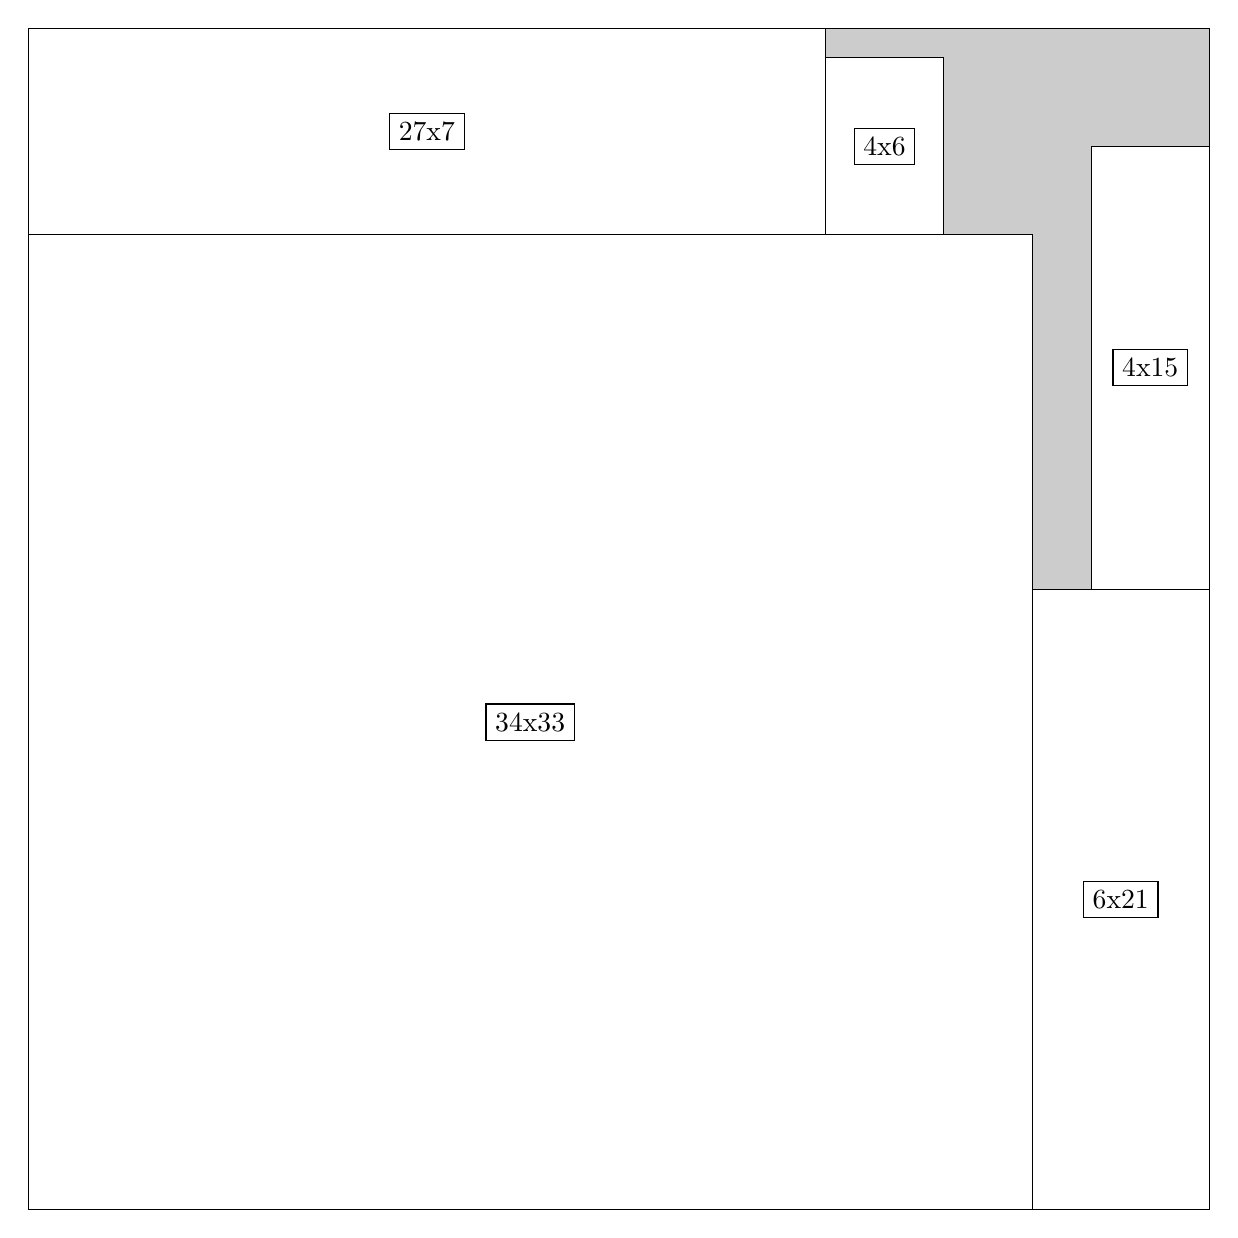
\begin{tikzpicture}[shorten >=1pt,scale=1.0,every node/.style={scale=1.0},->]
\tikzstyle{vertex}=[circle,fill=black!25,minimum size=14pt,inner sep=0pt]
\filldraw[fill=gray!40!white, draw=black] (0,0) rectangle (15.0,15.0);
\foreach \name/\x/\y/\w/\h in {34x33/0.0/0.0/12.75/12.375,27x7/0.0/12.375/10.125/2.625,6x21/12.75/0.0/2.25/7.875,4x15/13.5/7.875/1.5/5.625,4x6/10.125/12.375/1.5/2.25}
\filldraw[fill=white!40!white, draw=black] (\x,\y) rectangle node[draw] (\name) {\name} ++(\w,\h);
\end{tikzpicture}


w =34 , h =33 , x =0 , y =0 , v =1122
\par
w =27 , h =7 , x =0 , y =33 , v =189
\par
w =6 , h =21 , x =34 , y =0 , v =126
\par
w =4 , h =15 , x =36 , y =21 , v =60
\par
w =4 , h =6 , x =27 , y =33 , v =24
\par
\newpage


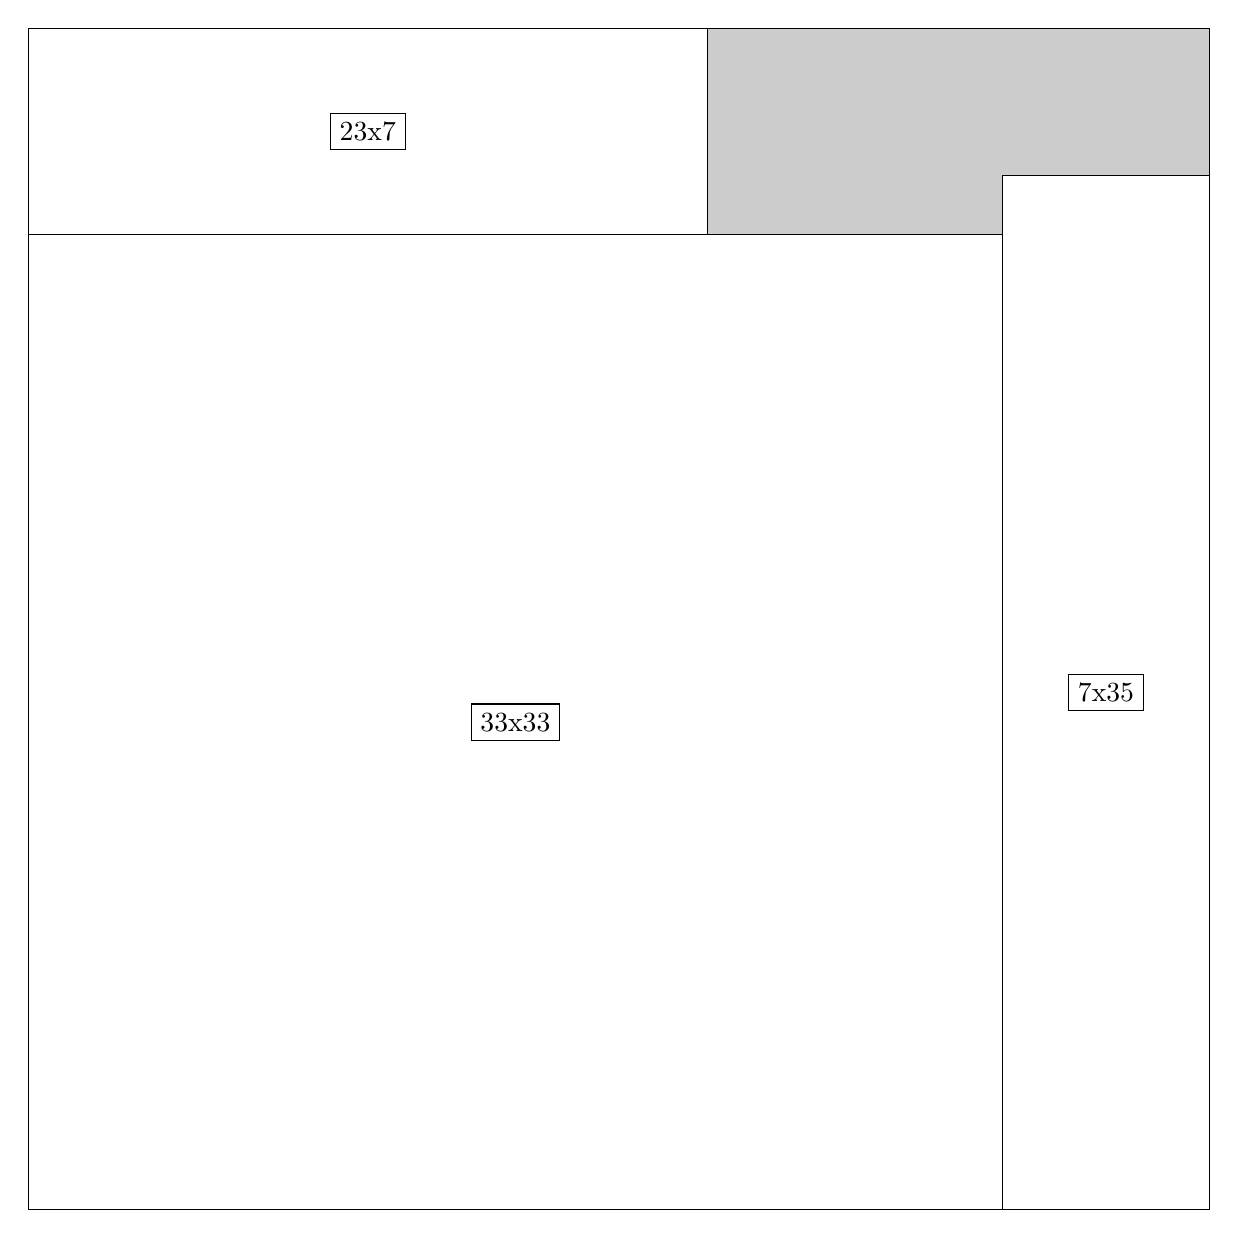
\begin{tikzpicture}[shorten >=1pt,scale=1.0,every node/.style={scale=1.0},->]
\tikzstyle{vertex}=[circle,fill=black!25,minimum size=14pt,inner sep=0pt]
\filldraw[fill=gray!40!white, draw=black] (0,0) rectangle (15.0,15.0);
\foreach \name/\x/\y/\w/\h in {33x33/0.0/0.0/12.375/12.375,7x35/12.375/0.0/2.625/13.125,23x7/0.0/12.375/8.625/2.625}
\filldraw[fill=white!40!white, draw=black] (\x,\y) rectangle node[draw] (\name) {\name} ++(\w,\h);
\end{tikzpicture}


w =33 , h =33 , x =0 , y =0 , v =1089
\par
w =7 , h =35 , x =33 , y =0 , v =245
\par
w =23 , h =7 , x =0 , y =33 , v =161
\par
\newpage


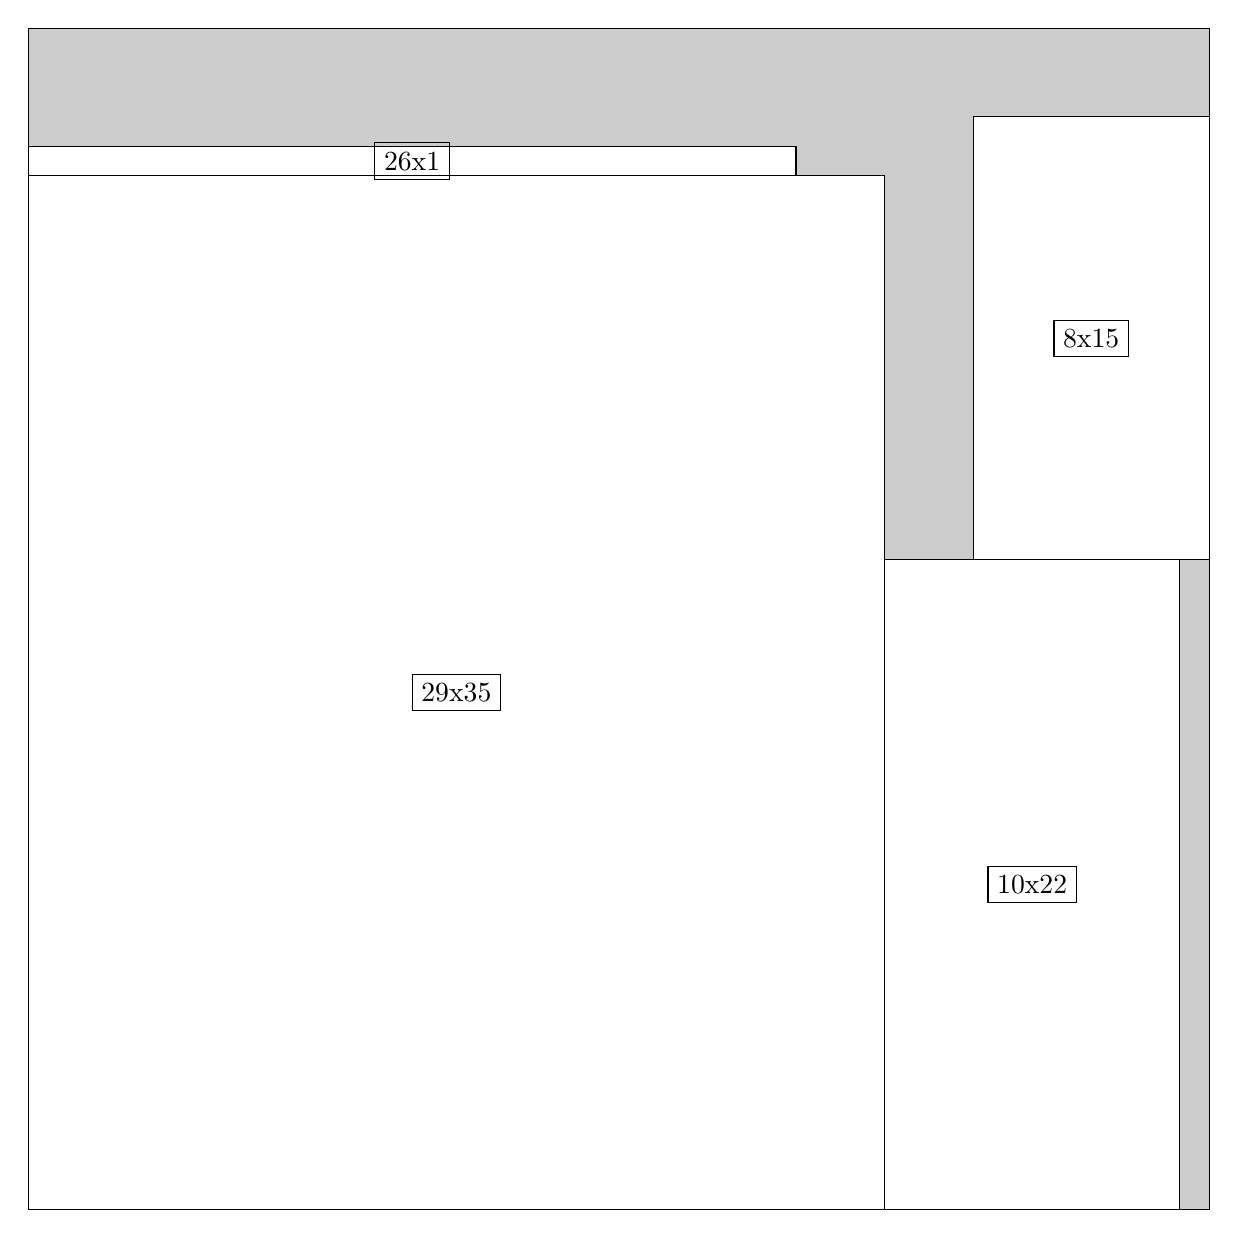
\begin{tikzpicture}[shorten >=1pt,scale=1.0,every node/.style={scale=1.0},->]
\tikzstyle{vertex}=[circle,fill=black!25,minimum size=14pt,inner sep=0pt]
\filldraw[fill=gray!40!white, draw=black] (0,0) rectangle (15.0,15.0);
\foreach \name/\x/\y/\w/\h in {29x35/0.0/0.0/10.875/13.125,8x15/12.0/8.25/3.0/5.625,10x22/10.875/0.0/3.75/8.25,26x1/0.0/13.125/9.75/0.375}
\filldraw[fill=white!40!white, draw=black] (\x,\y) rectangle node[draw] (\name) {\name} ++(\w,\h);
\end{tikzpicture}


w =29 , h =35 , x =0 , y =0 , v =1015
\par
w =8 , h =15 , x =32 , y =22 , v =120
\par
w =10 , h =22 , x =29 , y =0 , v =220
\par
w =26 , h =1 , x =0 , y =35 , v =26
\par
\newpage


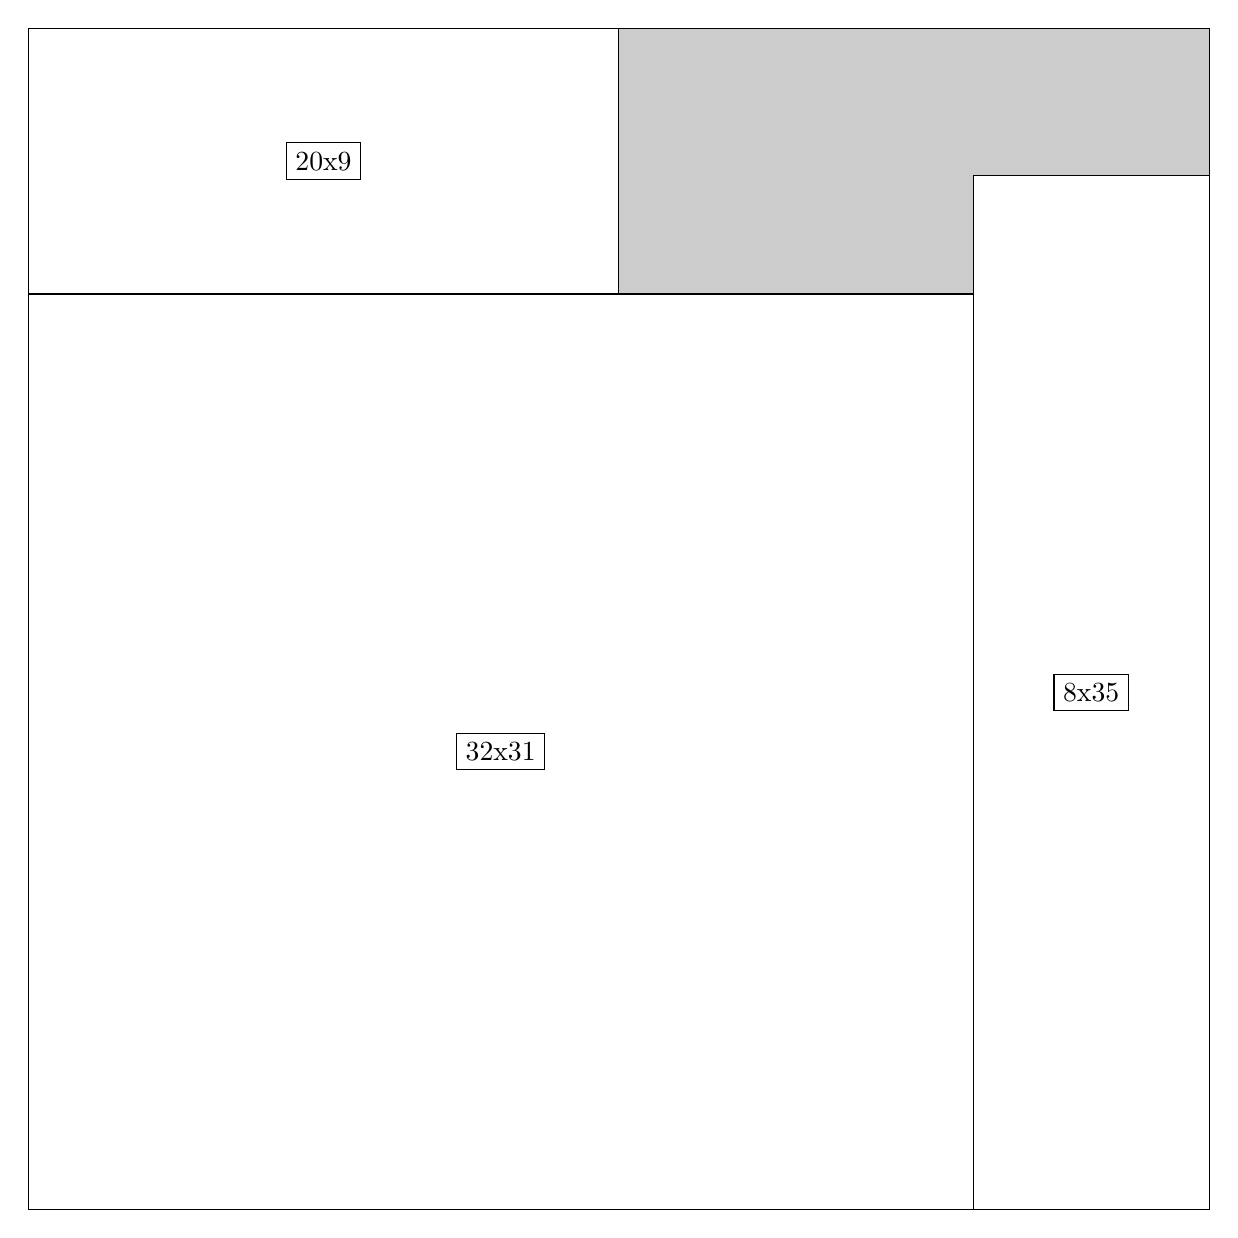
\begin{tikzpicture}[shorten >=1pt,scale=1.0,every node/.style={scale=1.0},->]
\tikzstyle{vertex}=[circle,fill=black!25,minimum size=14pt,inner sep=0pt]
\filldraw[fill=gray!40!white, draw=black] (0,0) rectangle (15.0,15.0);
\foreach \name/\x/\y/\w/\h in {32x31/0.0/0.0/12.0/11.625,8x35/12.0/0.0/3.0/13.125,20x9/0.0/11.625/7.5/3.375}
\filldraw[fill=white!40!white, draw=black] (\x,\y) rectangle node[draw] (\name) {\name} ++(\w,\h);
\end{tikzpicture}


w =32 , h =31 , x =0 , y =0 , v =992
\par
w =8 , h =35 , x =32 , y =0 , v =280
\par
w =20 , h =9 , x =0 , y =31 , v =180
\par
\newpage


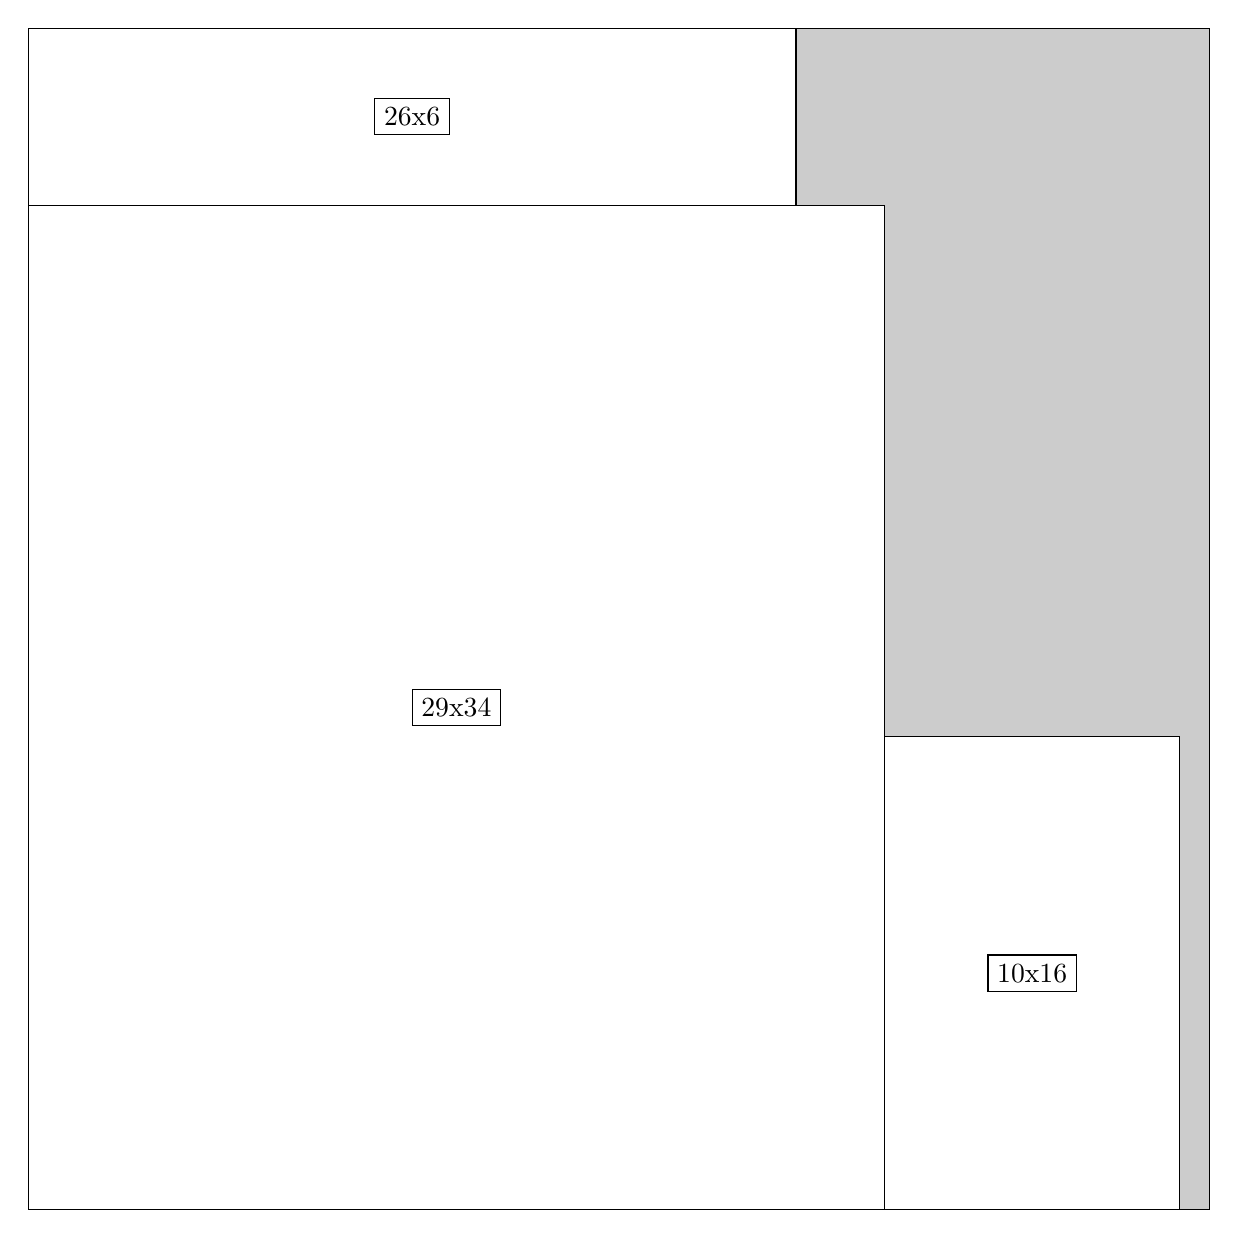
\begin{tikzpicture}[shorten >=1pt,scale=1.0,every node/.style={scale=1.0},->]
\tikzstyle{vertex}=[circle,fill=black!25,minimum size=14pt,inner sep=0pt]
\filldraw[fill=gray!40!white, draw=black] (0,0) rectangle (15.0,15.0);
\foreach \name/\x/\y/\w/\h in {29x34/0.0/0.0/10.875/12.75,10x16/10.875/0.0/3.75/6.0,26x6/0.0/12.75/9.75/2.25}
\filldraw[fill=white!40!white, draw=black] (\x,\y) rectangle node[draw] (\name) {\name} ++(\w,\h);
\end{tikzpicture}


w =29 , h =34 , x =0 , y =0 , v =986
\par
w =10 , h =16 , x =29 , y =0 , v =160
\par
w =26 , h =6 , x =0 , y =34 , v =156
\par
\newpage


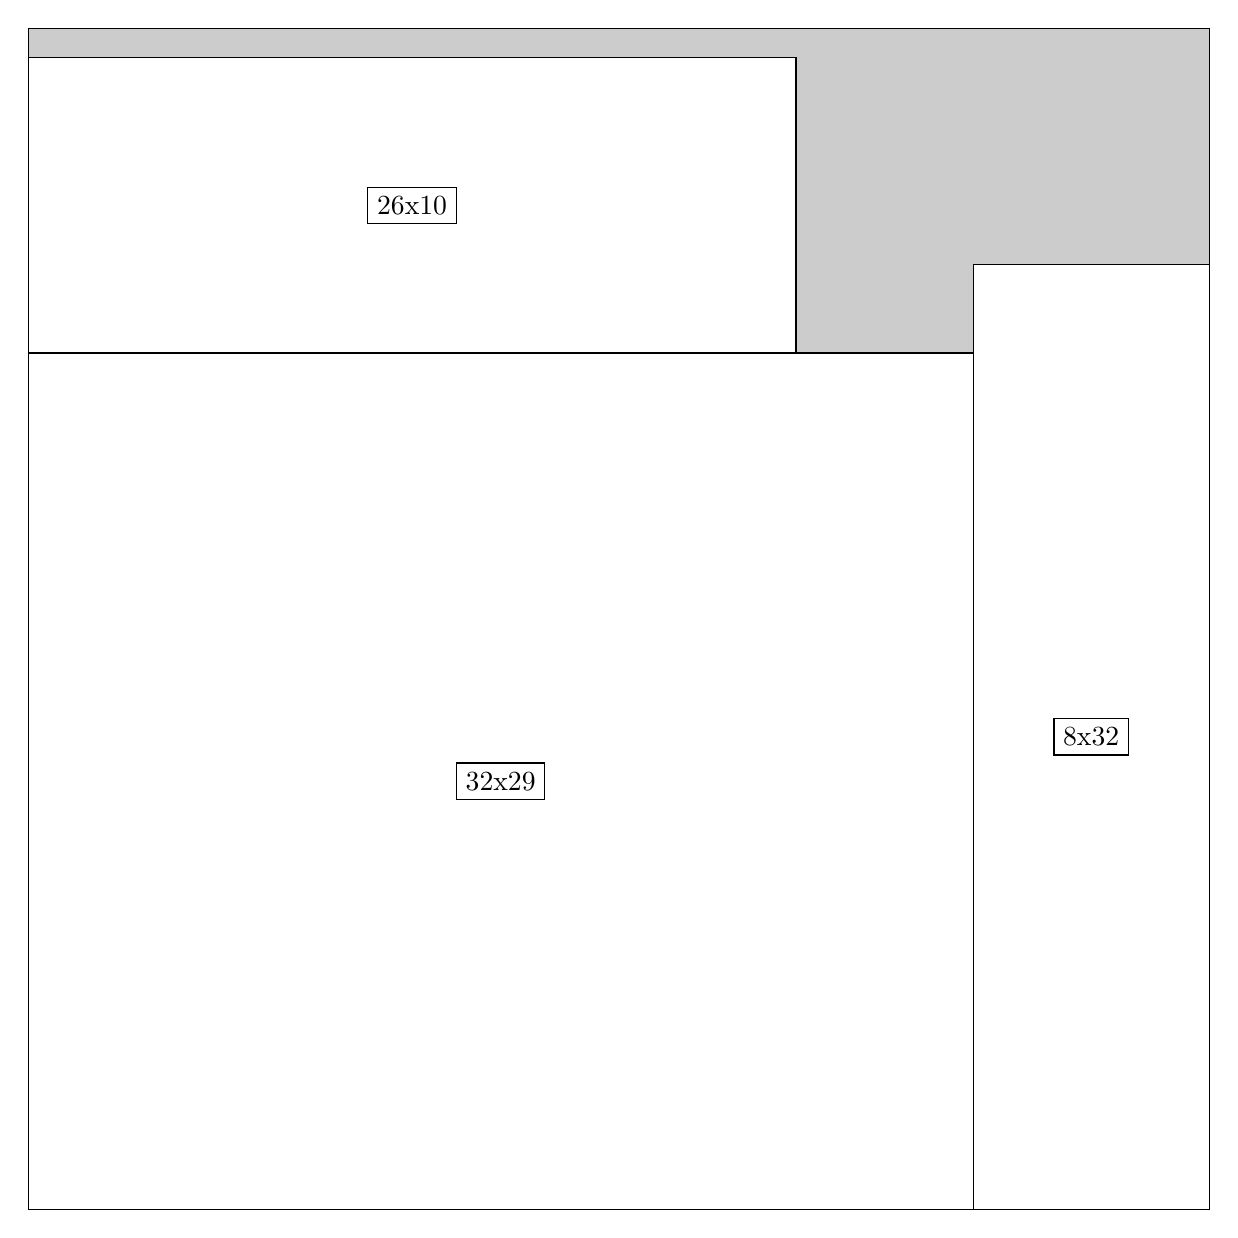
\begin{tikzpicture}[shorten >=1pt,scale=1.0,every node/.style={scale=1.0},->]
\tikzstyle{vertex}=[circle,fill=black!25,minimum size=14pt,inner sep=0pt]
\filldraw[fill=gray!40!white, draw=black] (0,0) rectangle (15.0,15.0);
\foreach \name/\x/\y/\w/\h in {32x29/0.0/0.0/12.0/10.875,26x10/0.0/10.875/9.75/3.75,8x32/12.0/0.0/3.0/12.0}
\filldraw[fill=white!40!white, draw=black] (\x,\y) rectangle node[draw] (\name) {\name} ++(\w,\h);
\end{tikzpicture}


w =32 , h =29 , x =0 , y =0 , v =928
\par
w =26 , h =10 , x =0 , y =29 , v =260
\par
w =8 , h =32 , x =32 , y =0 , v =256
\par
\newpage


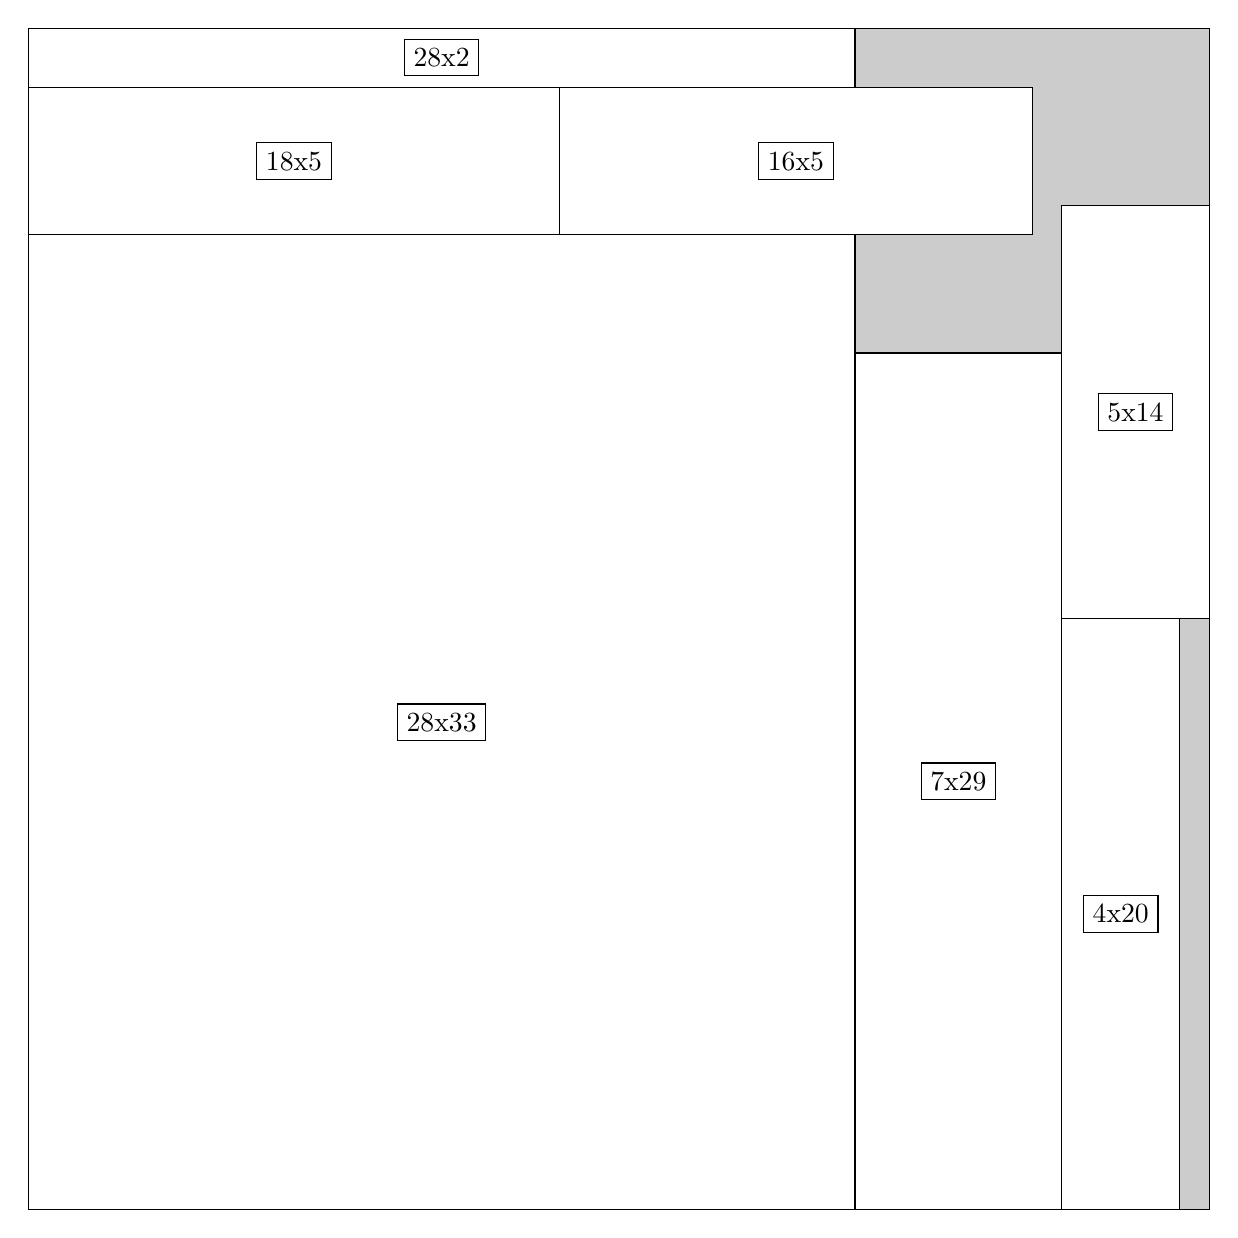
\begin{tikzpicture}[shorten >=1pt,scale=1.0,every node/.style={scale=1.0},->]
\tikzstyle{vertex}=[circle,fill=black!25,minimum size=14pt,inner sep=0pt]
\filldraw[fill=gray!40!white, draw=black] (0,0) rectangle (15.0,15.0);
\foreach \name/\x/\y/\w/\h in {28x33/0.0/0.0/10.5/12.375,7x29/10.5/0.0/2.625/10.875,18x5/0.0/12.375/6.75/1.875,16x5/6.75/12.375/6.0/1.875,4x20/13.125/0.0/1.5/7.5,5x14/13.125/7.5/1.875/5.25,28x2/0.0/14.25/10.5/0.75}
\filldraw[fill=white!40!white, draw=black] (\x,\y) rectangle node[draw] (\name) {\name} ++(\w,\h);
\end{tikzpicture}


w =28 , h =33 , x =0 , y =0 , v =924
\par
w =7 , h =29 , x =28 , y =0 , v =203
\par
w =18 , h =5 , x =0 , y =33 , v =90
\par
w =16 , h =5 , x =18 , y =33 , v =80
\par
w =4 , h =20 , x =35 , y =0 , v =80
\par
w =5 , h =14 , x =35 , y =20 , v =70
\par
w =28 , h =2 , x =0 , y =38 , v =56
\par
\newpage


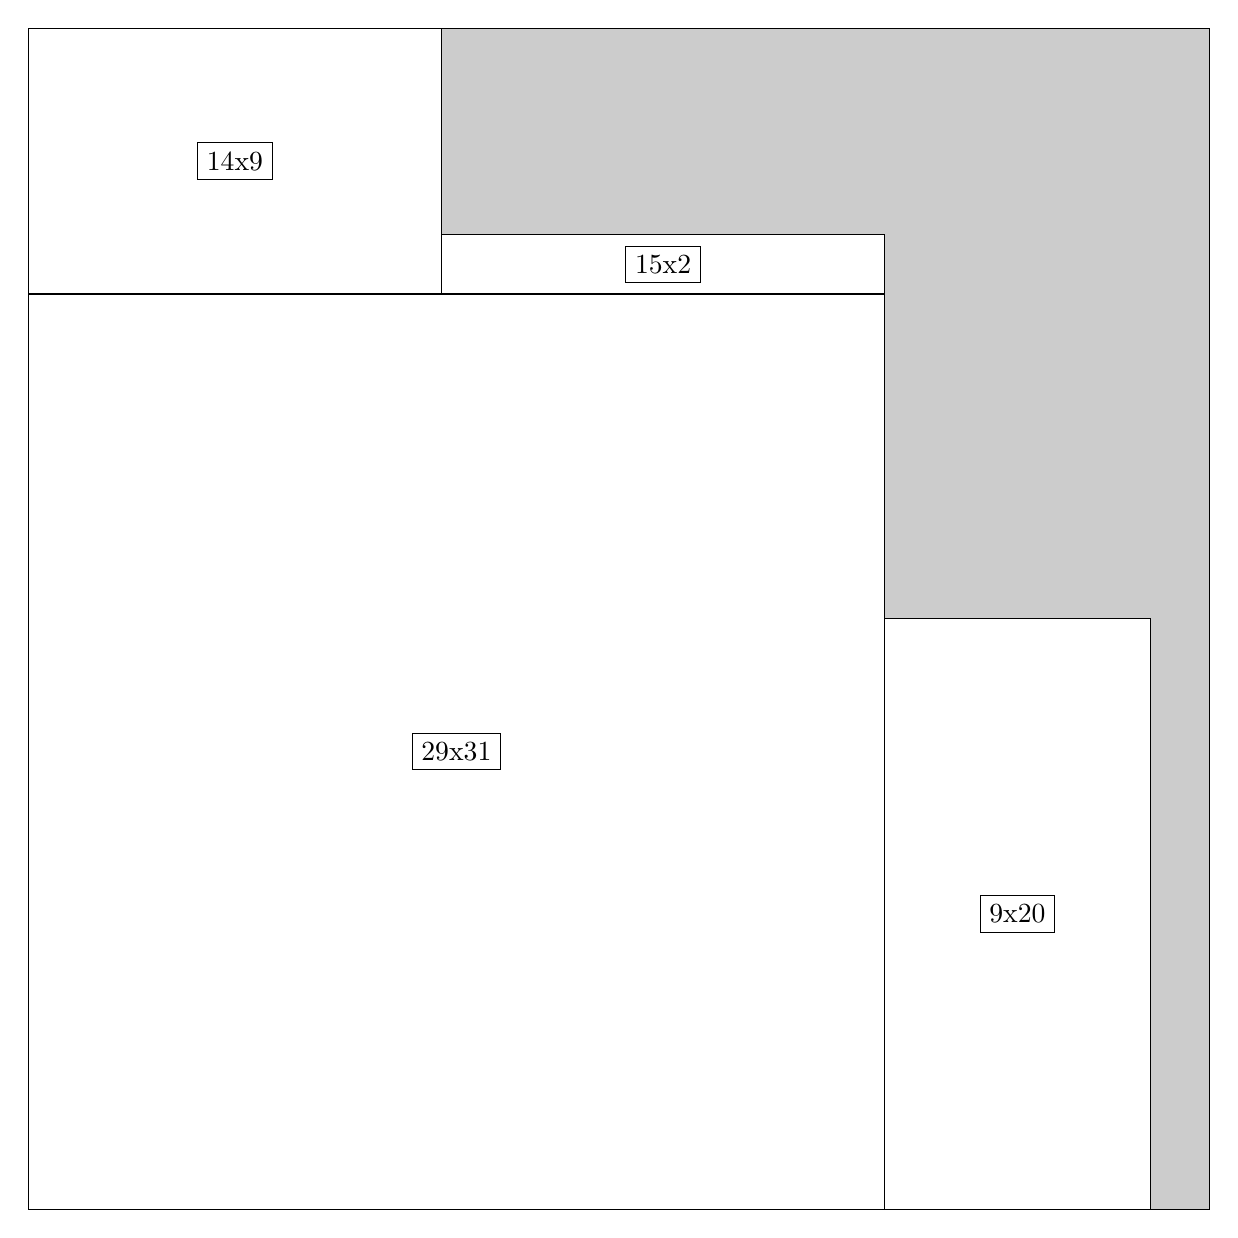
\begin{tikzpicture}[shorten >=1pt,scale=1.0,every node/.style={scale=1.0},->]
\tikzstyle{vertex}=[circle,fill=black!25,minimum size=14pt,inner sep=0pt]
\filldraw[fill=gray!40!white, draw=black] (0,0) rectangle (15.0,15.0);
\foreach \name/\x/\y/\w/\h in {29x31/0.0/0.0/10.875/11.625,9x20/10.875/0.0/3.375/7.5,14x9/0.0/11.625/5.25/3.375,15x2/5.25/11.625/5.625/0.75}
\filldraw[fill=white!40!white, draw=black] (\x,\y) rectangle node[draw] (\name) {\name} ++(\w,\h);
\end{tikzpicture}


w =29 , h =31 , x =0 , y =0 , v =899
\par
w =9 , h =20 , x =29 , y =0 , v =180
\par
w =14 , h =9 , x =0 , y =31 , v =126
\par
w =15 , h =2 , x =14 , y =31 , v =30
\par
\newpage


\begin{tikzpicture}[shorten >=1pt,scale=1.0,every node/.style={scale=1.0},->]
\tikzstyle{vertex}=[circle,fill=black!25,minimum size=14pt,inner sep=0pt]
\filldraw[fill=gray!40!white, draw=black] (0,0) rectangle (15.0,15.0);
\foreach \name/\x/\y/\w/\h in {32x28/0.0/0.0/12.0/10.5,8x28/12.0/0.0/3.0/10.5,18x12/8.25/10.5/6.75/4.5,17x12/1.875/10.5/6.375/4.5,5x9/0.0/10.5/1.875/3.375,2x2/0.0/13.875/0.75/0.75}
\filldraw[fill=white!40!white, draw=black] (\x,\y) rectangle node[draw] (\name) {\name} ++(\w,\h);
\end{tikzpicture}


w =32 , h =28 , x =0 , y =0 , v =896
\par
w =8 , h =28 , x =32 , y =0 , v =224
\par
w =18 , h =12 , x =22 , y =28 , v =216
\par
w =17 , h =12 , x =5 , y =28 , v =204
\par
w =5 , h =9 , x =0 , y =28 , v =45
\par
w =2 , h =2 , x =0 , y =37 , v =4
\par
\newpage


\begin{tikzpicture}[shorten >=1pt,scale=1.0,every node/.style={scale=1.0},->]
\tikzstyle{vertex}=[circle,fill=black!25,minimum size=14pt,inner sep=0pt]
\filldraw[fill=gray!40!white, draw=black] (0,0) rectangle (15.0,15.0);
\foreach \name/\x/\y/\w/\h in {35x25/0.0/0.0/13.125/9.375,35x15/0.0/9.375/13.125/5.625,5x28/13.125/0.0/1.875/10.5,5x7/13.125/10.5/1.875/2.625,5x3/13.125/13.125/1.875/1.125}
\filldraw[fill=white!40!white, draw=black] (\x,\y) rectangle node[draw] (\name) {\name} ++(\w,\h);
\end{tikzpicture}


w =35 , h =25 , x =0 , y =0 , v =875
\par
w =35 , h =15 , x =0 , y =25 , v =525
\par
w =5 , h =28 , x =35 , y =0 , v =140
\par
w =5 , h =7 , x =35 , y =28 , v =35
\par
w =5 , h =3 , x =35 , y =35 , v =15
\par
\newpage


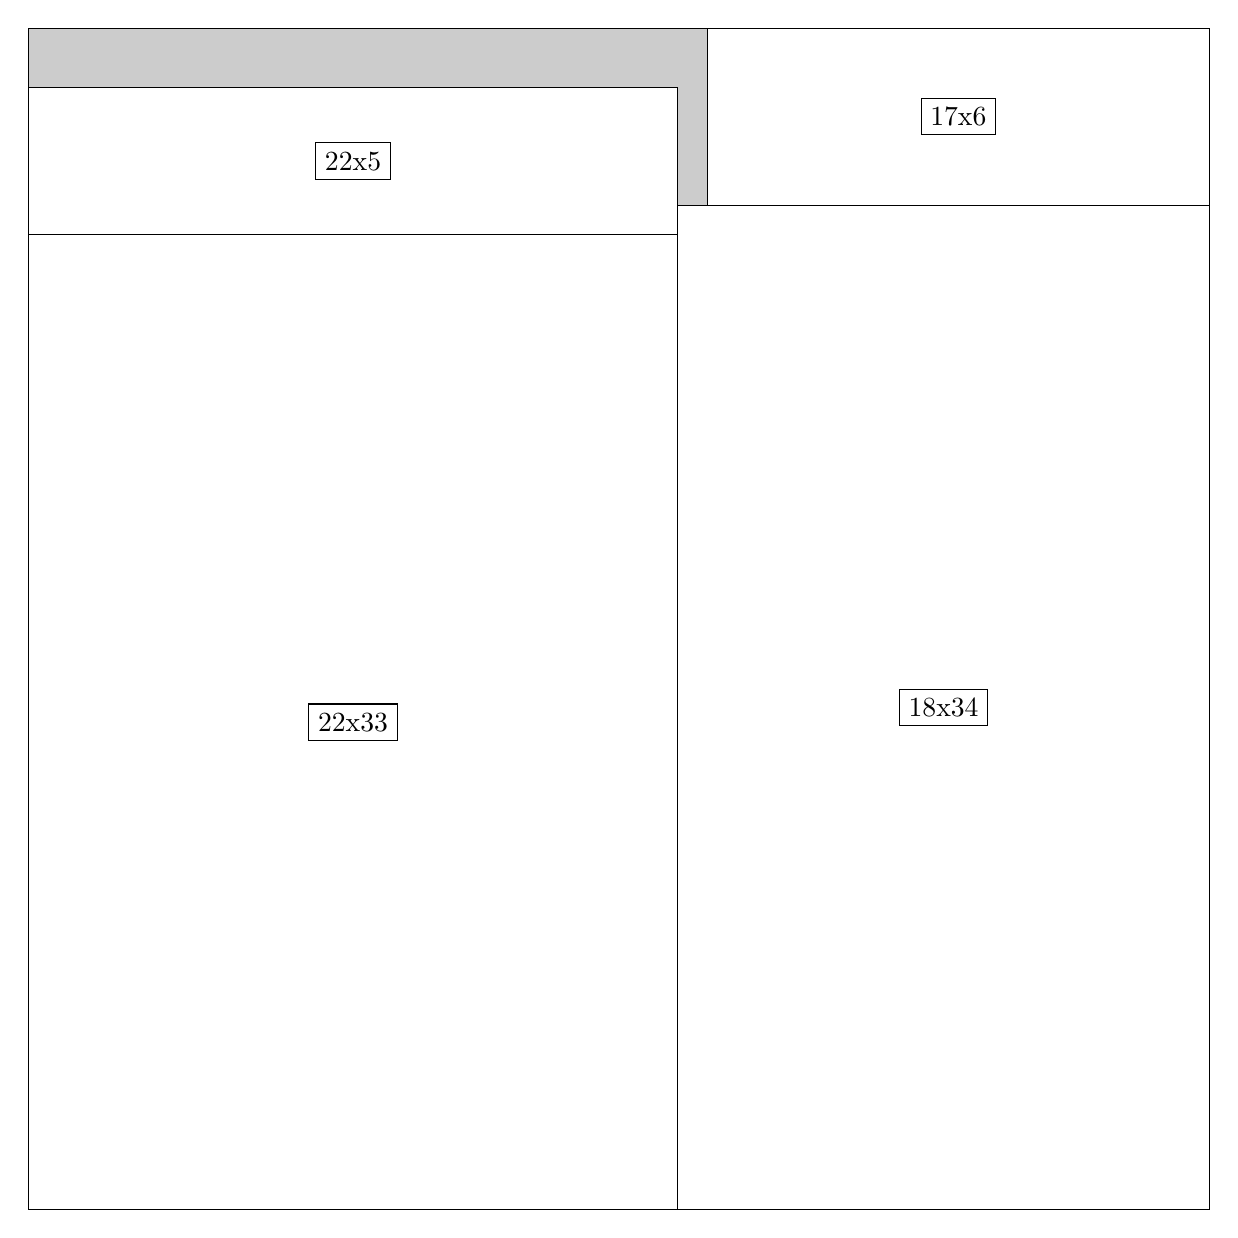
\begin{tikzpicture}[shorten >=1pt,scale=1.0,every node/.style={scale=1.0},->]
\tikzstyle{vertex}=[circle,fill=black!25,minimum size=14pt,inner sep=0pt]
\filldraw[fill=gray!40!white, draw=black] (0,0) rectangle (15.0,15.0);
\foreach \name/\x/\y/\w/\h in {22x33/0.0/0.0/8.25/12.375,18x34/8.25/0.0/6.75/12.75,22x5/0.0/12.375/8.25/1.875,17x6/8.625/12.75/6.375/2.25}
\filldraw[fill=white!40!white, draw=black] (\x,\y) rectangle node[draw] (\name) {\name} ++(\w,\h);
\end{tikzpicture}


w =22 , h =33 , x =0 , y =0 , v =726
\par
w =18 , h =34 , x =22 , y =0 , v =612
\par
w =22 , h =5 , x =0 , y =33 , v =110
\par
w =17 , h =6 , x =23 , y =34 , v =102
\par
\newpage


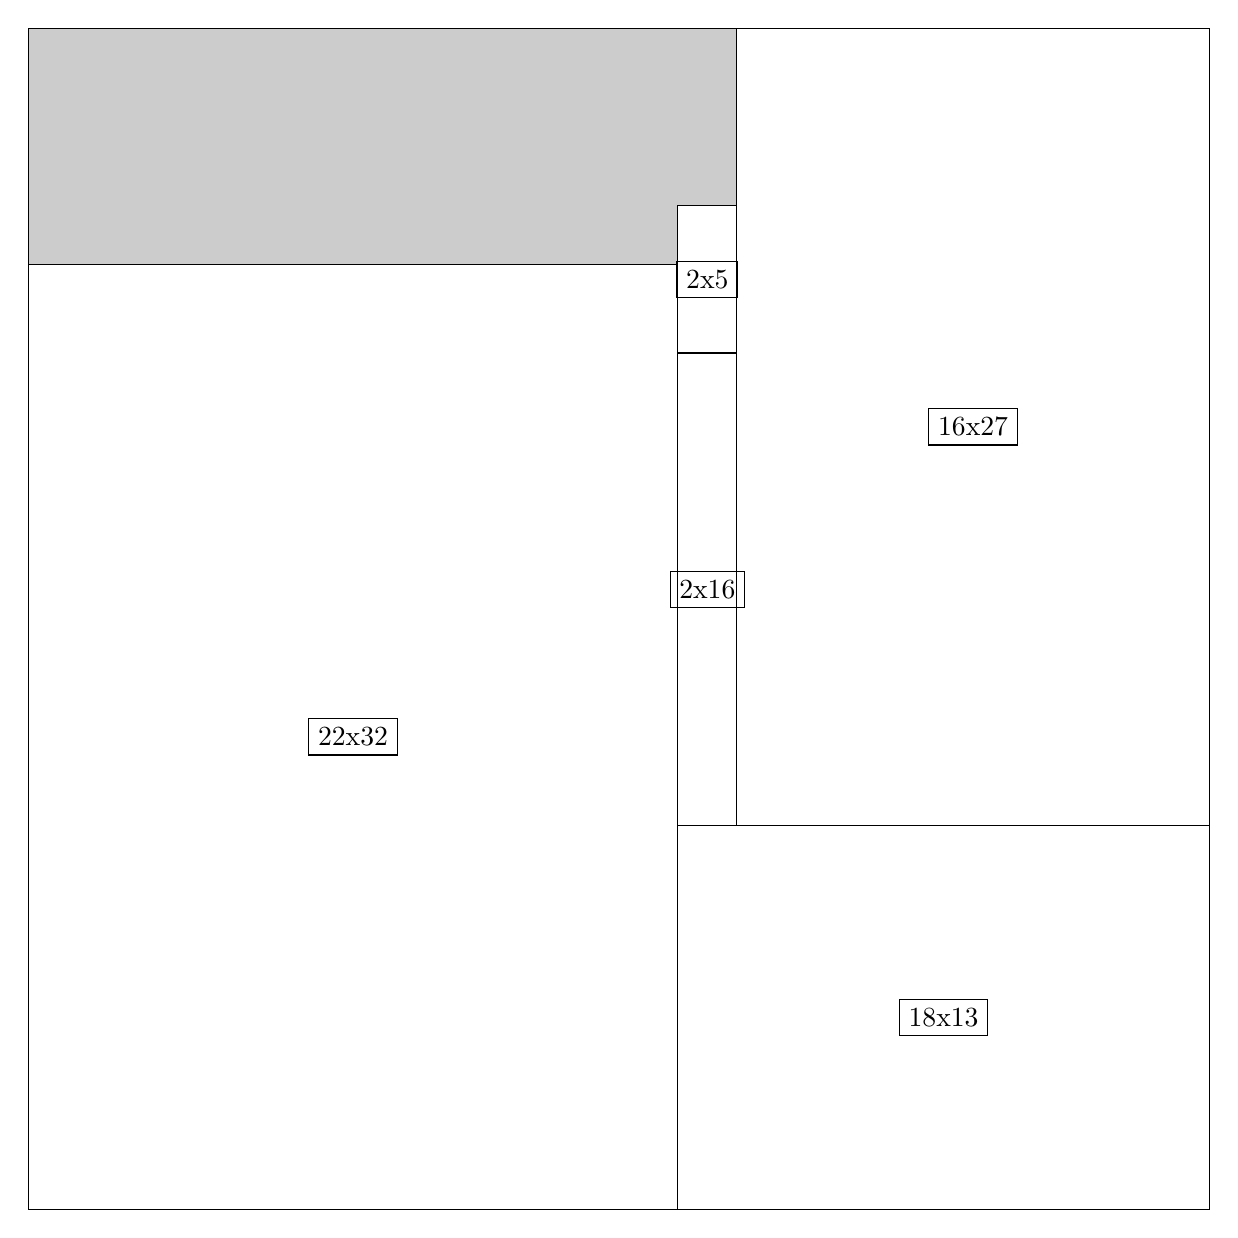
\begin{tikzpicture}[shorten >=1pt,scale=1.0,every node/.style={scale=1.0},->]
\tikzstyle{vertex}=[circle,fill=black!25,minimum size=14pt,inner sep=0pt]
\filldraw[fill=gray!40!white, draw=black] (0,0) rectangle (15.0,15.0);
\foreach \name/\x/\y/\w/\h in {22x32/0.0/0.0/8.25/12.0,16x27/9.0/4.875/6.0/10.125,18x13/8.25/0.0/6.75/4.875,2x16/8.25/4.875/0.75/6.0,2x5/8.25/10.875/0.75/1.875}
\filldraw[fill=white!40!white, draw=black] (\x,\y) rectangle node[draw] (\name) {\name} ++(\w,\h);
\end{tikzpicture}


w =22 , h =32 , x =0 , y =0 , v =704
\par
w =16 , h =27 , x =24 , y =13 , v =432
\par
w =18 , h =13 , x =22 , y =0 , v =234
\par
w =2 , h =16 , x =22 , y =13 , v =32
\par
w =2 , h =5 , x =22 , y =29 , v =10
\par
\newpage


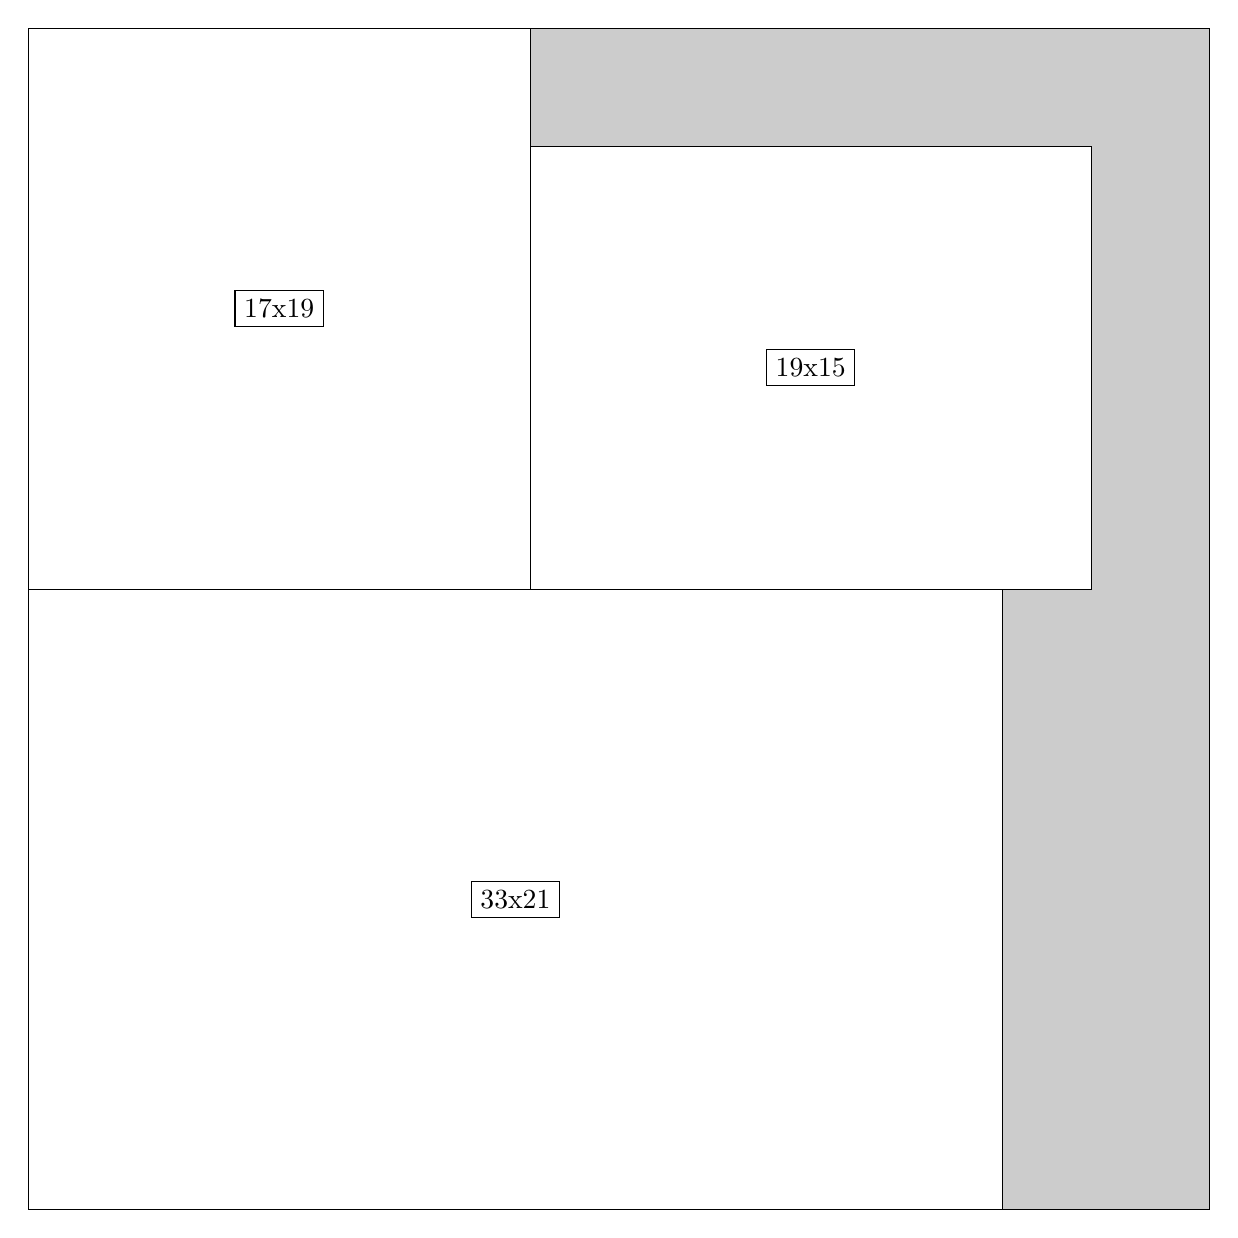
\begin{tikzpicture}[shorten >=1pt,scale=1.0,every node/.style={scale=1.0},->]
\tikzstyle{vertex}=[circle,fill=black!25,minimum size=14pt,inner sep=0pt]
\filldraw[fill=gray!40!white, draw=black] (0,0) rectangle (15.0,15.0);
\foreach \name/\x/\y/\w/\h in {33x21/0.0/0.0/12.375/7.875,17x19/0.0/7.875/6.375/7.125,19x15/6.375/7.875/7.125/5.625}
\filldraw[fill=white!40!white, draw=black] (\x,\y) rectangle node[draw] (\name) {\name} ++(\w,\h);
\end{tikzpicture}


w =33 , h =21 , x =0 , y =0 , v =693
\par
w =17 , h =19 , x =0 , y =21 , v =323
\par
w =19 , h =15 , x =17 , y =21 , v =285
\par
\newpage


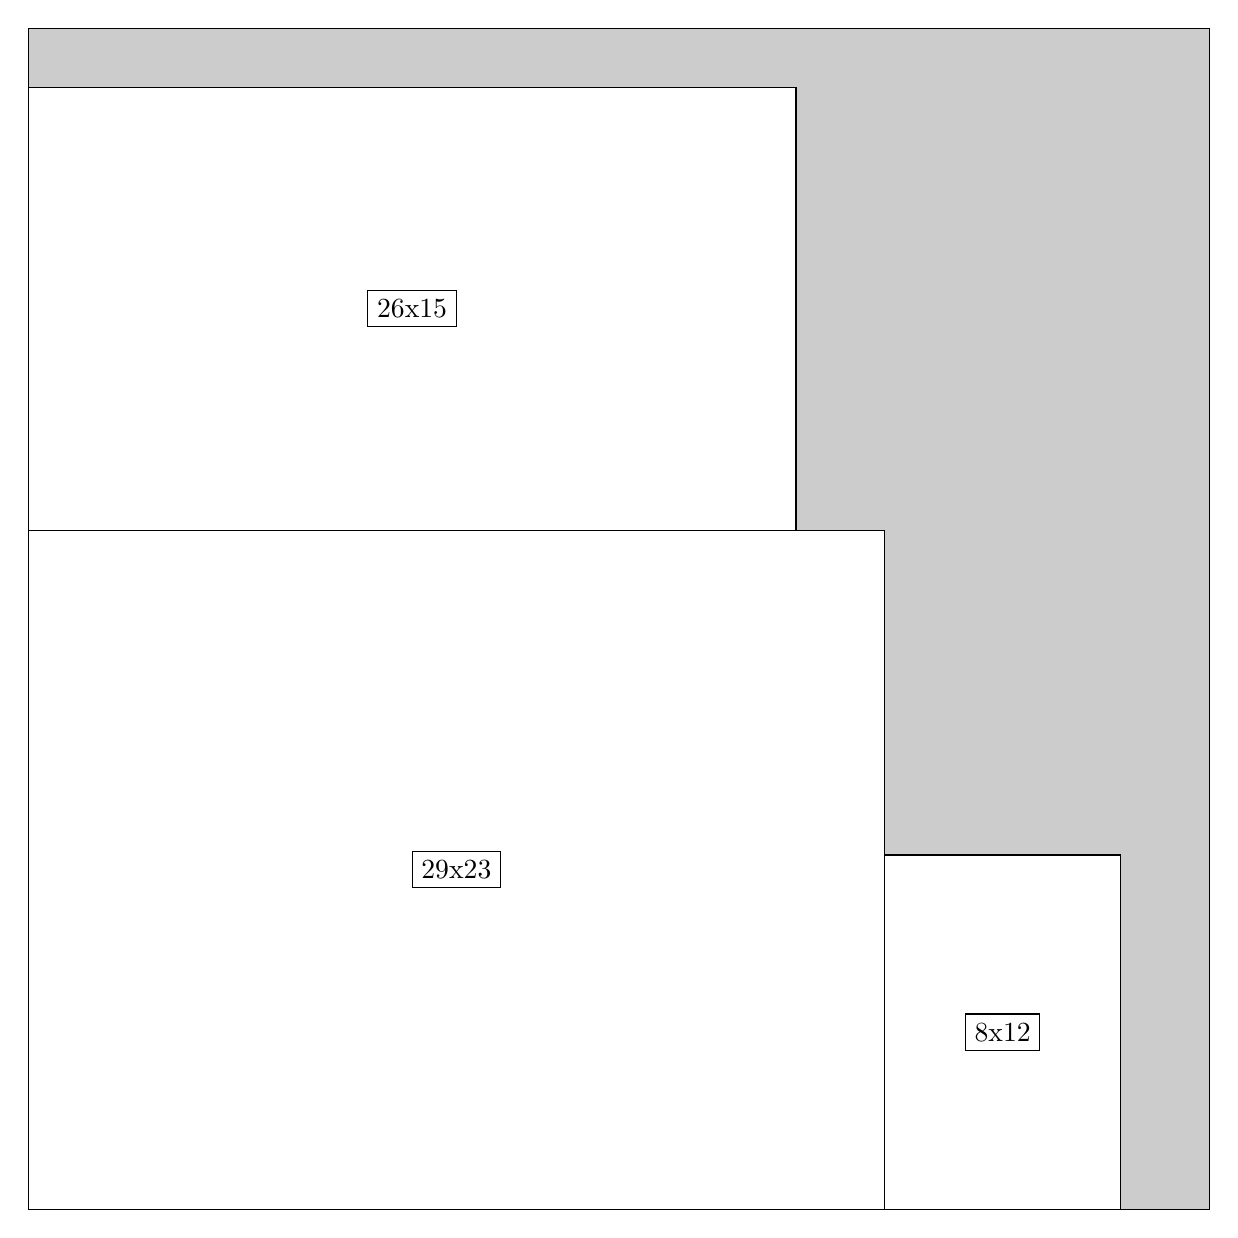
\begin{tikzpicture}[shorten >=1pt,scale=1.0,every node/.style={scale=1.0},->]
\tikzstyle{vertex}=[circle,fill=black!25,minimum size=14pt,inner sep=0pt]
\filldraw[fill=gray!40!white, draw=black] (0,0) rectangle (15.0,15.0);
\foreach \name/\x/\y/\w/\h in {29x23/0.0/0.0/10.875/8.625,26x15/0.0/8.625/9.75/5.625,8x12/10.875/0.0/3.0/4.5}
\filldraw[fill=white!40!white, draw=black] (\x,\y) rectangle node[draw] (\name) {\name} ++(\w,\h);
\end{tikzpicture}


w =29 , h =23 , x =0 , y =0 , v =667
\par
w =26 , h =15 , x =0 , y =23 , v =390
\par
w =8 , h =12 , x =29 , y =0 , v =96
\par
\newpage


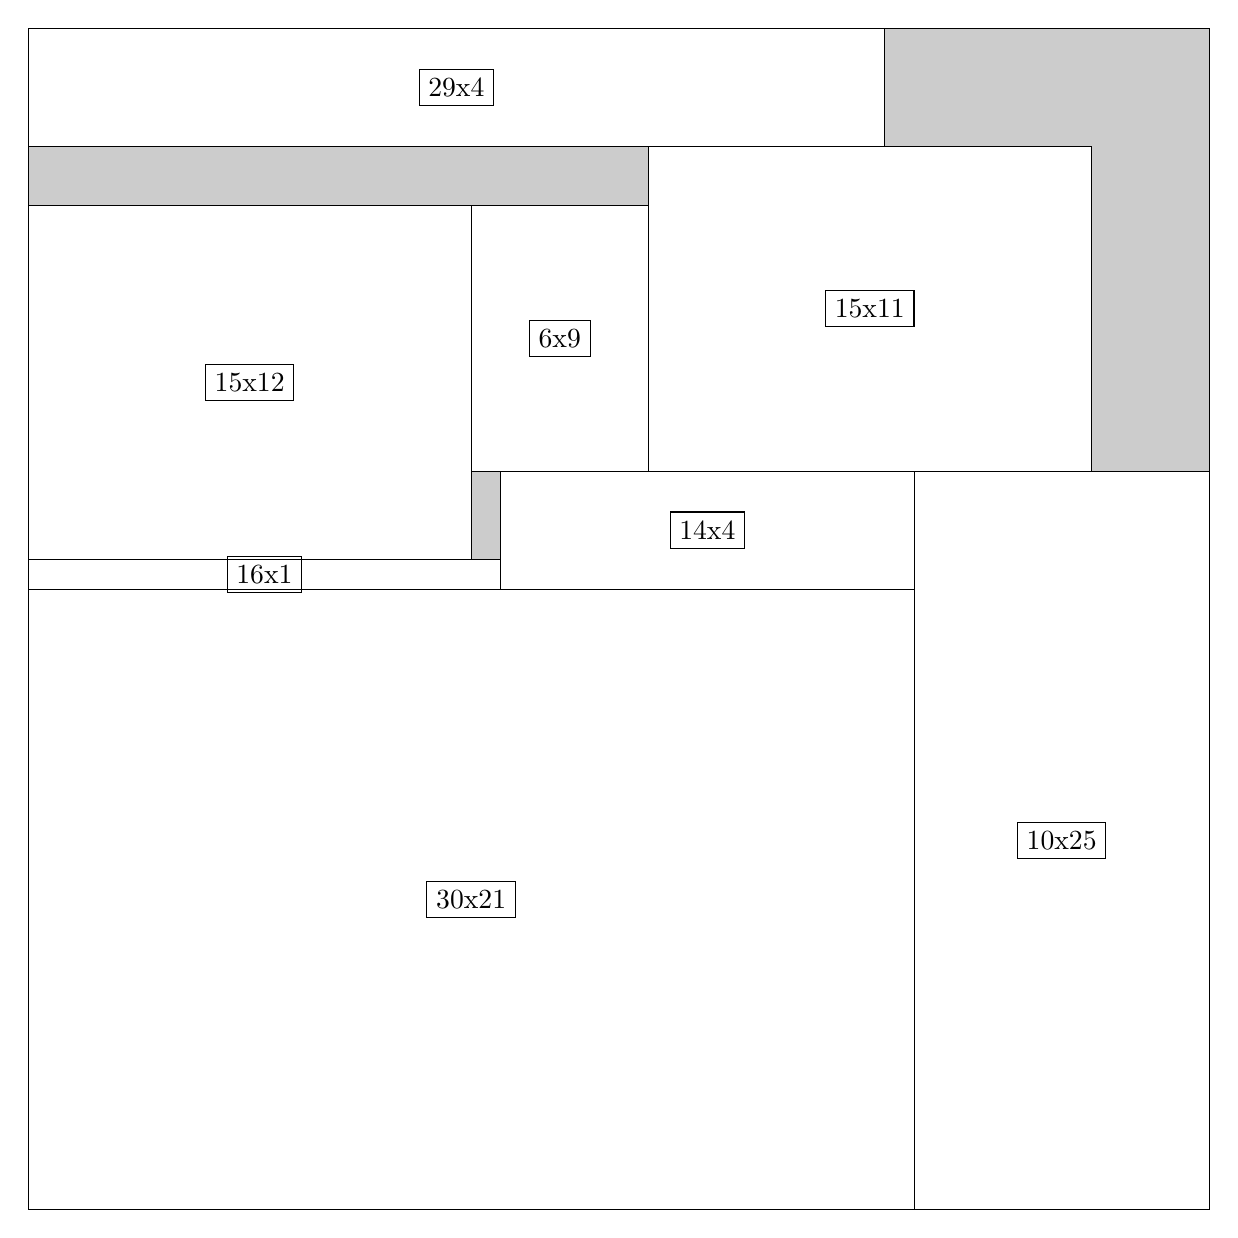
\begin{tikzpicture}[shorten >=1pt,scale=1.0,every node/.style={scale=1.0},->]
\tikzstyle{vertex}=[circle,fill=black!25,minimum size=14pt,inner sep=0pt]
\filldraw[fill=gray!40!white, draw=black] (0,0) rectangle (15.0,15.0);
\foreach \name/\x/\y/\w/\h in {30x21/0.0/0.0/11.25/7.875,15x12/0.0/8.25/5.625/4.5,15x11/7.875/9.375/5.625/4.125,10x25/11.25/0.0/3.75/9.375,29x4/0.0/13.5/10.875/1.5,14x4/6.0/7.875/5.25/1.5,6x9/5.625/9.375/2.25/3.375,16x1/0.0/7.875/6.0/0.375}
\filldraw[fill=white!40!white, draw=black] (\x,\y) rectangle node[draw] (\name) {\name} ++(\w,\h);
\end{tikzpicture}


w =30 , h =21 , x =0 , y =0 , v =630
\par
w =15 , h =12 , x =0 , y =22 , v =180
\par
w =15 , h =11 , x =21 , y =25 , v =165
\par
w =10 , h =25 , x =30 , y =0 , v =250
\par
w =29 , h =4 , x =0 , y =36 , v =116
\par
w =14 , h =4 , x =16 , y =21 , v =56
\par
w =6 , h =9 , x =15 , y =25 , v =54
\par
w =16 , h =1 , x =0 , y =21 , v =16
\par
\newpage


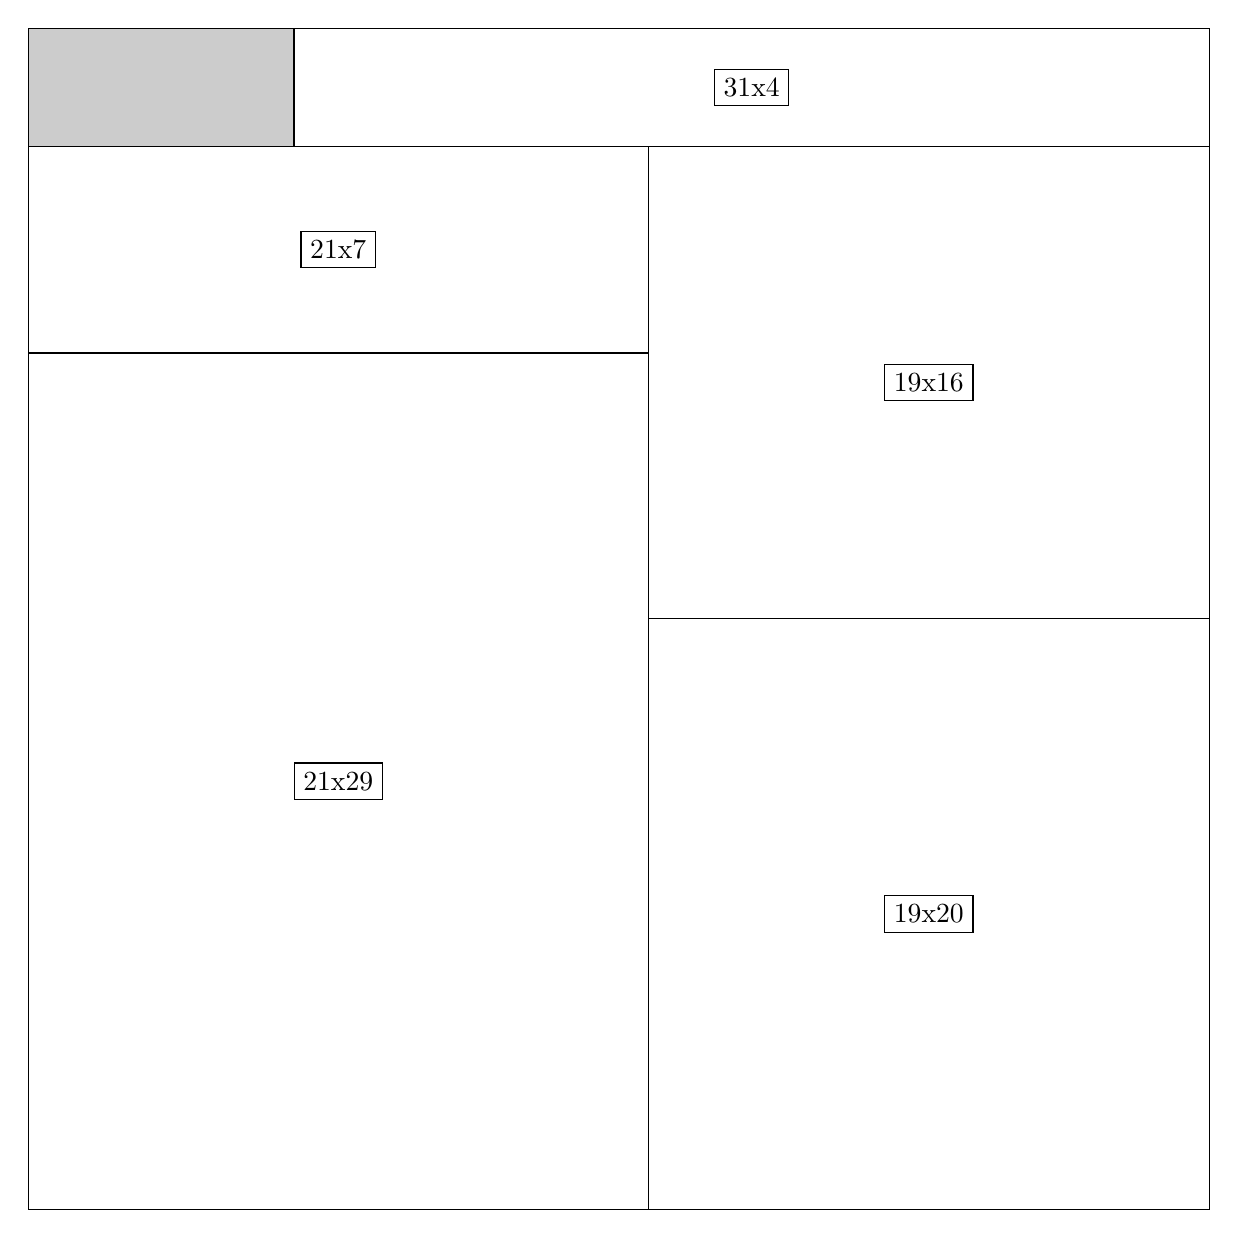
\begin{tikzpicture}[shorten >=1pt,scale=1.0,every node/.style={scale=1.0},->]
\tikzstyle{vertex}=[circle,fill=black!25,minimum size=14pt,inner sep=0pt]
\filldraw[fill=gray!40!white, draw=black] (0,0) rectangle (15.0,15.0);
\foreach \name/\x/\y/\w/\h in {21x29/0.0/0.0/7.875/10.875,19x20/7.875/0.0/7.125/7.5,19x16/7.875/7.5/7.125/6.0,21x7/0.0/10.875/7.875/2.625,31x4/3.375/13.5/11.625/1.5}
\filldraw[fill=white!40!white, draw=black] (\x,\y) rectangle node[draw] (\name) {\name} ++(\w,\h);
\end{tikzpicture}


w =21 , h =29 , x =0 , y =0 , v =609
\par
w =19 , h =20 , x =21 , y =0 , v =380
\par
w =19 , h =16 , x =21 , y =20 , v =304
\par
w =21 , h =7 , x =0 , y =29 , v =147
\par
w =31 , h =4 , x =9 , y =36 , v =124
\par
\newpage


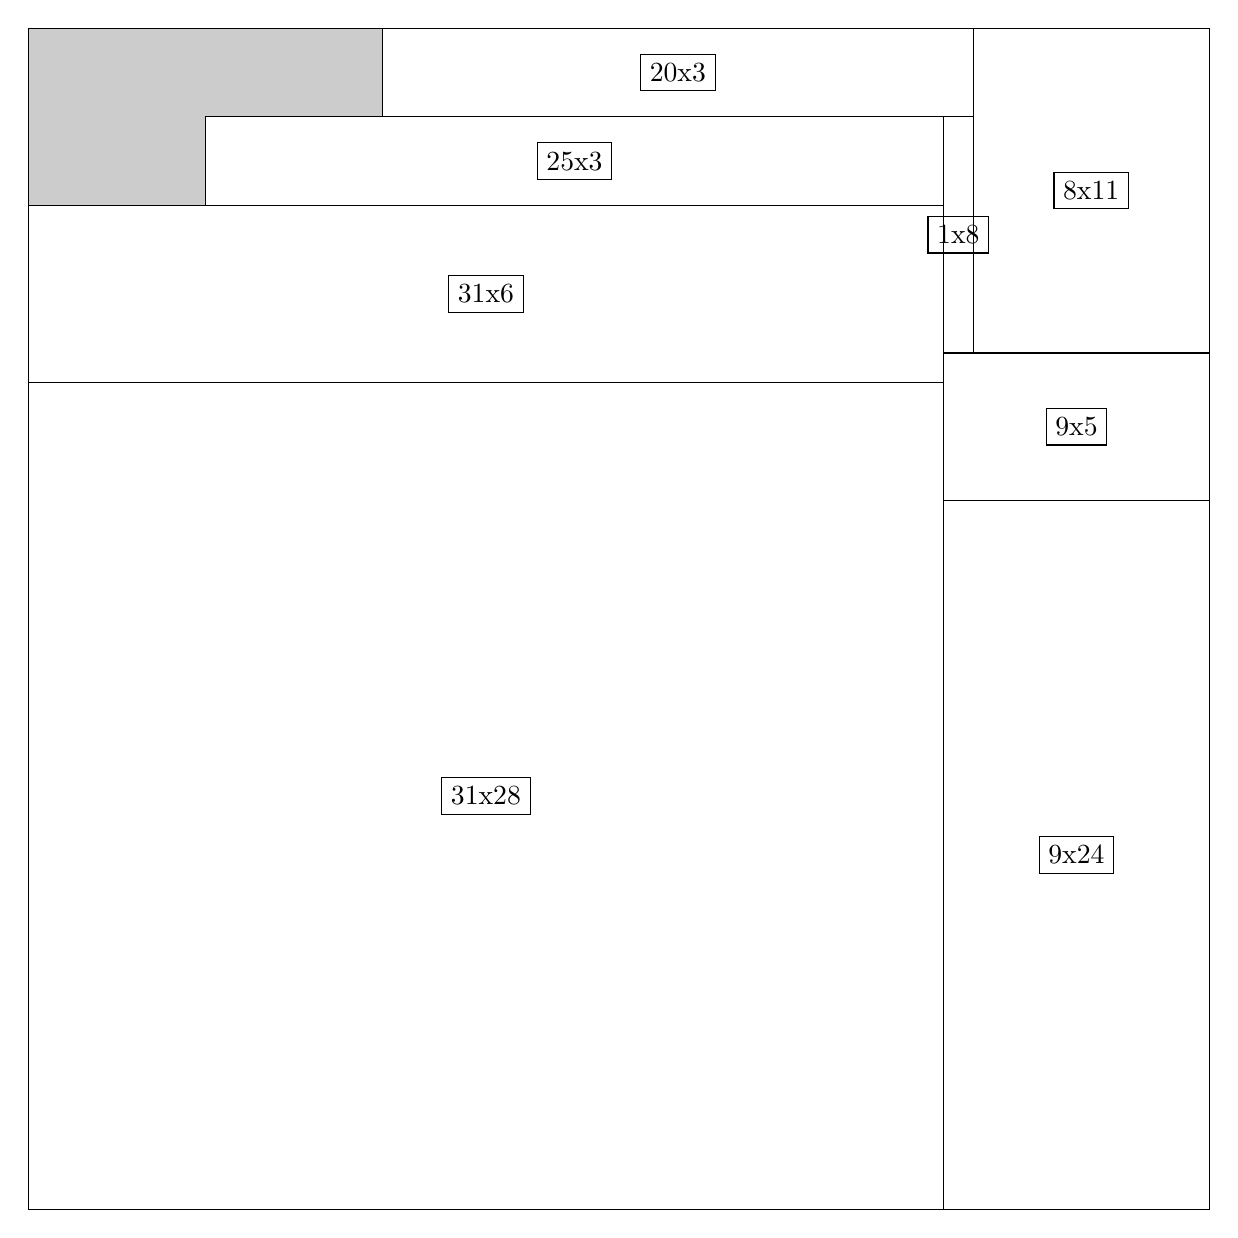
\begin{tikzpicture}[shorten >=1pt,scale=1.0,every node/.style={scale=1.0},->]
\tikzstyle{vertex}=[circle,fill=black!25,minimum size=14pt,inner sep=0pt]
\filldraw[fill=gray!40!white, draw=black] (0,0) rectangle (15.0,15.0);
\foreach \name/\x/\y/\w/\h in {31x28/0.0/0.0/11.625/10.5,9x24/11.625/0.0/3.375/9.0,31x6/0.0/10.5/11.625/2.25,8x11/12.0/10.875/3.0/4.125,25x3/2.25/12.75/9.375/1.125,20x3/4.5/13.875/7.5/1.125,9x5/11.625/9.0/3.375/1.875,1x8/11.625/10.875/0.375/3.0}
\filldraw[fill=white!40!white, draw=black] (\x,\y) rectangle node[draw] (\name) {\name} ++(\w,\h);
\end{tikzpicture}


w =31 , h =28 , x =0 , y =0 , v =868
\par
w =9 , h =24 , x =31 , y =0 , v =216
\par
w =31 , h =6 , x =0 , y =28 , v =186
\par
w =8 , h =11 , x =32 , y =29 , v =88
\par
w =25 , h =3 , x =6 , y =34 , v =75
\par
w =20 , h =3 , x =12 , y =37 , v =60
\par
w =9 , h =5 , x =31 , y =24 , v =45
\par
w =1 , h =8 , x =31 , y =29 , v =8
\par
\newpage


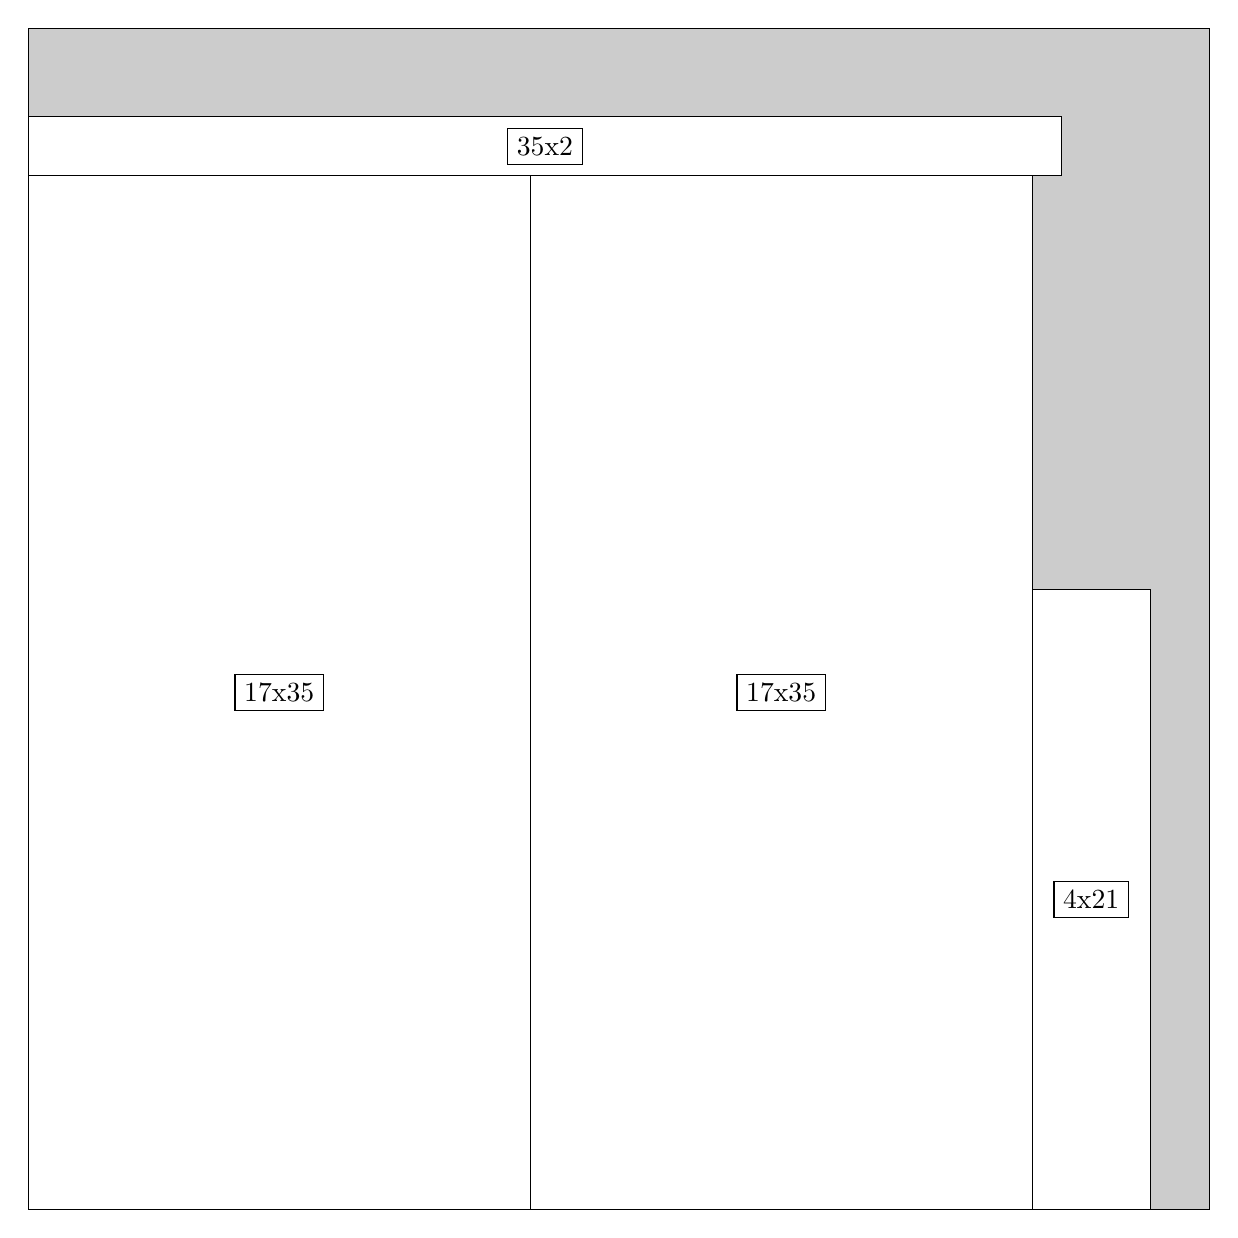
\begin{tikzpicture}[shorten >=1pt,scale=1.0,every node/.style={scale=1.0},->]
\tikzstyle{vertex}=[circle,fill=black!25,minimum size=14pt,inner sep=0pt]
\filldraw[fill=gray!40!white, draw=black] (0,0) rectangle (15.0,15.0);
\foreach \name/\x/\y/\w/\h in {17x35/0.0/0.0/6.375/13.125,17x35/6.375/0.0/6.375/13.125,4x21/12.75/0.0/1.5/7.875,35x2/0.0/13.125/13.125/0.75}
\filldraw[fill=white!40!white, draw=black] (\x,\y) rectangle node[draw] (\name) {\name} ++(\w,\h);
\end{tikzpicture}


w =17 , h =35 , x =0 , y =0 , v =595
\par
w =17 , h =35 , x =17 , y =0 , v =595
\par
w =4 , h =21 , x =34 , y =0 , v =84
\par
w =35 , h =2 , x =0 , y =35 , v =70
\par
\newpage


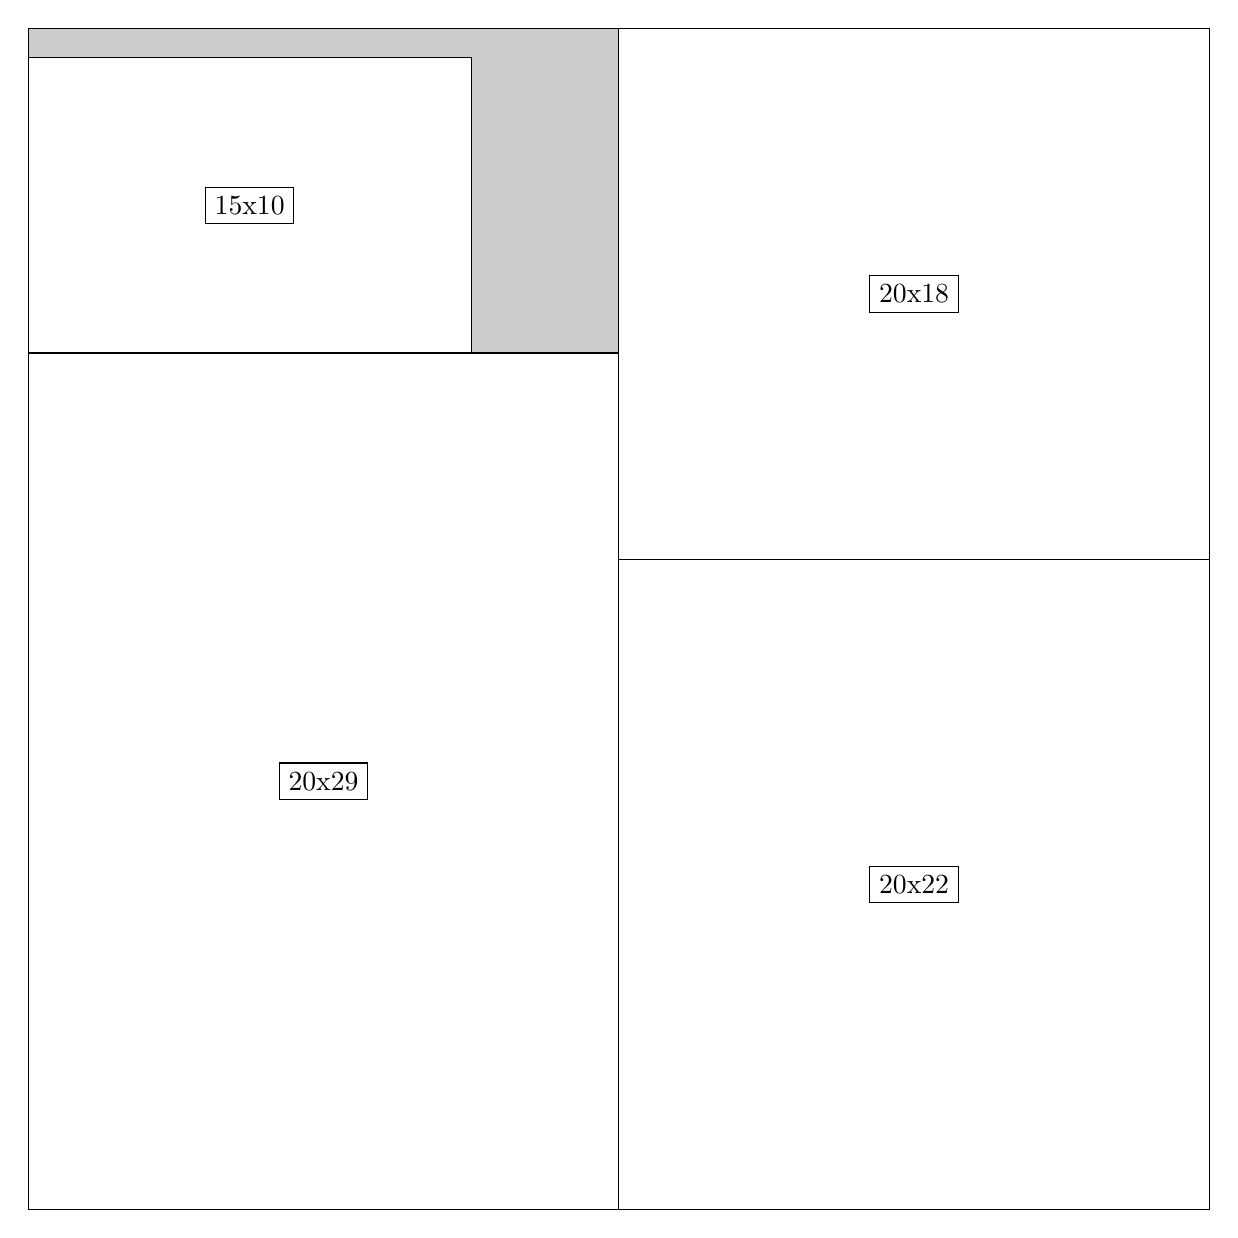
\begin{tikzpicture}[shorten >=1pt,scale=1.0,every node/.style={scale=1.0},->]
\tikzstyle{vertex}=[circle,fill=black!25,minimum size=14pt,inner sep=0pt]
\filldraw[fill=gray!40!white, draw=black] (0,0) rectangle (15.0,15.0);
\foreach \name/\x/\y/\w/\h in {20x29/0.0/0.0/7.5/10.875,20x22/7.5/0.0/7.5/8.25,20x18/7.5/8.25/7.5/6.75,15x10/0.0/10.875/5.625/3.75}
\filldraw[fill=white!40!white, draw=black] (\x,\y) rectangle node[draw] (\name) {\name} ++(\w,\h);
\end{tikzpicture}


w =20 , h =29 , x =0 , y =0 , v =580
\par
w =20 , h =22 , x =20 , y =0 , v =440
\par
w =20 , h =18 , x =20 , y =22 , v =360
\par
w =15 , h =10 , x =0 , y =29 , v =150
\par
\newpage


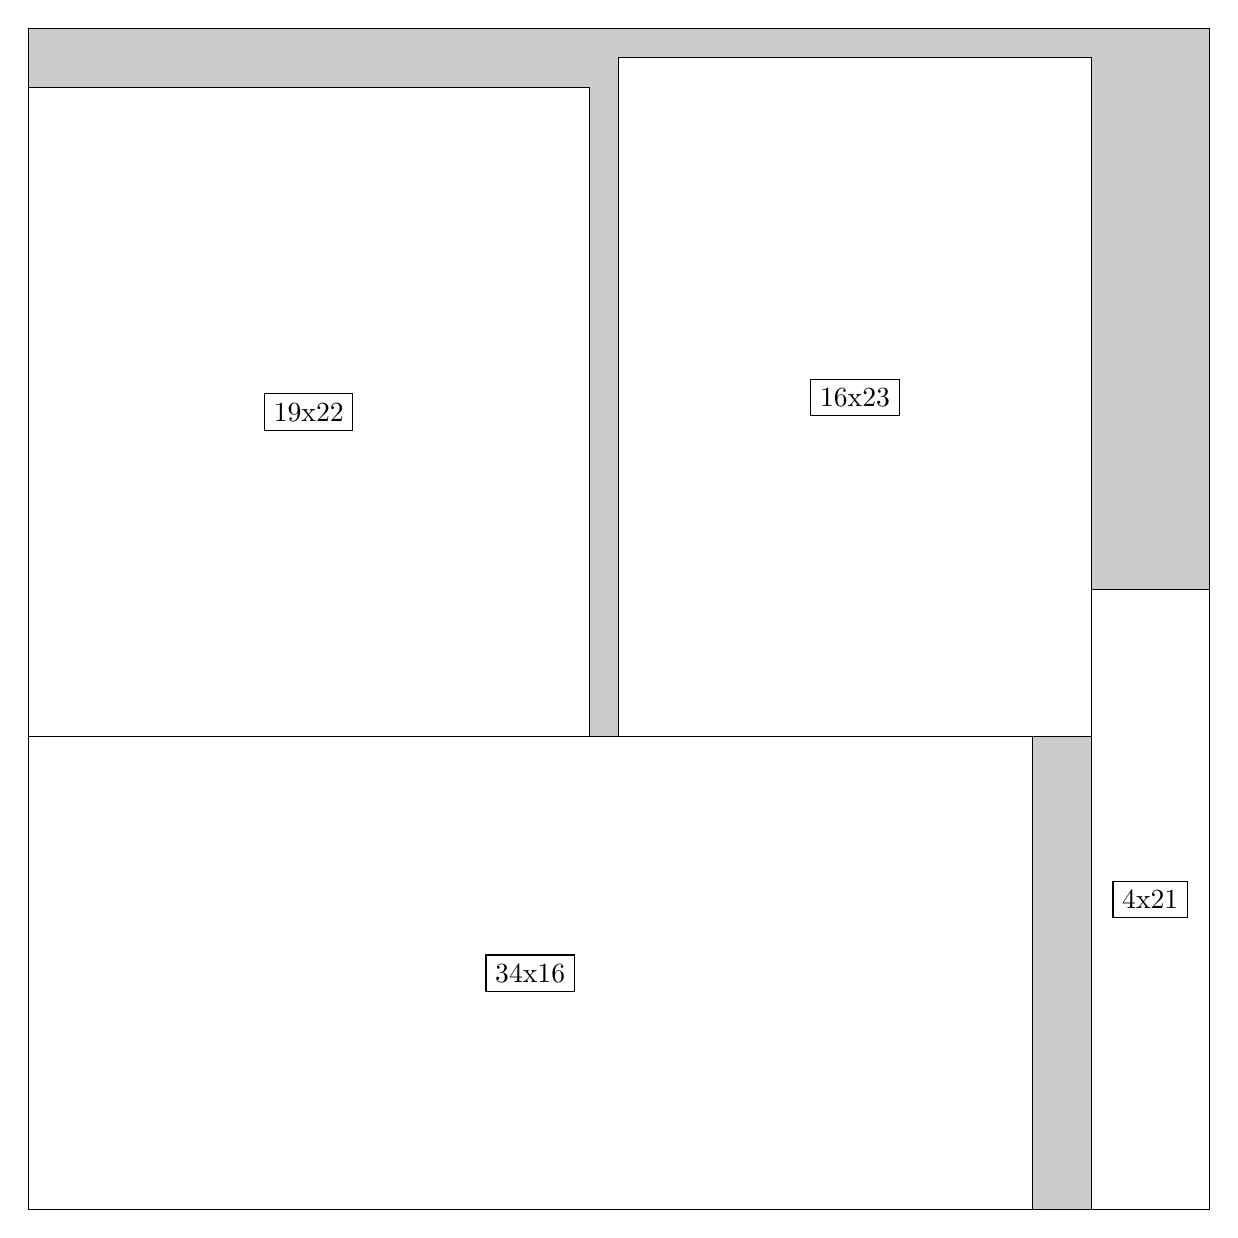
\begin{tikzpicture}[shorten >=1pt,scale=1.0,every node/.style={scale=1.0},->]
\tikzstyle{vertex}=[circle,fill=black!25,minimum size=14pt,inner sep=0pt]
\filldraw[fill=gray!40!white, draw=black] (0,0) rectangle (15.0,15.0);
\foreach \name/\x/\y/\w/\h in {34x16/0.0/0.0/12.75/6.0,19x22/0.0/6.0/7.125/8.25,16x23/7.5/6.0/6.0/8.625,4x21/13.5/0.0/1.5/7.875}
\filldraw[fill=white!40!white, draw=black] (\x,\y) rectangle node[draw] (\name) {\name} ++(\w,\h);
\end{tikzpicture}


w =34 , h =16 , x =0 , y =0 , v =544
\par
w =19 , h =22 , x =0 , y =16 , v =418
\par
w =16 , h =23 , x =20 , y =16 , v =368
\par
w =4 , h =21 , x =36 , y =0 , v =84
\par
\newpage


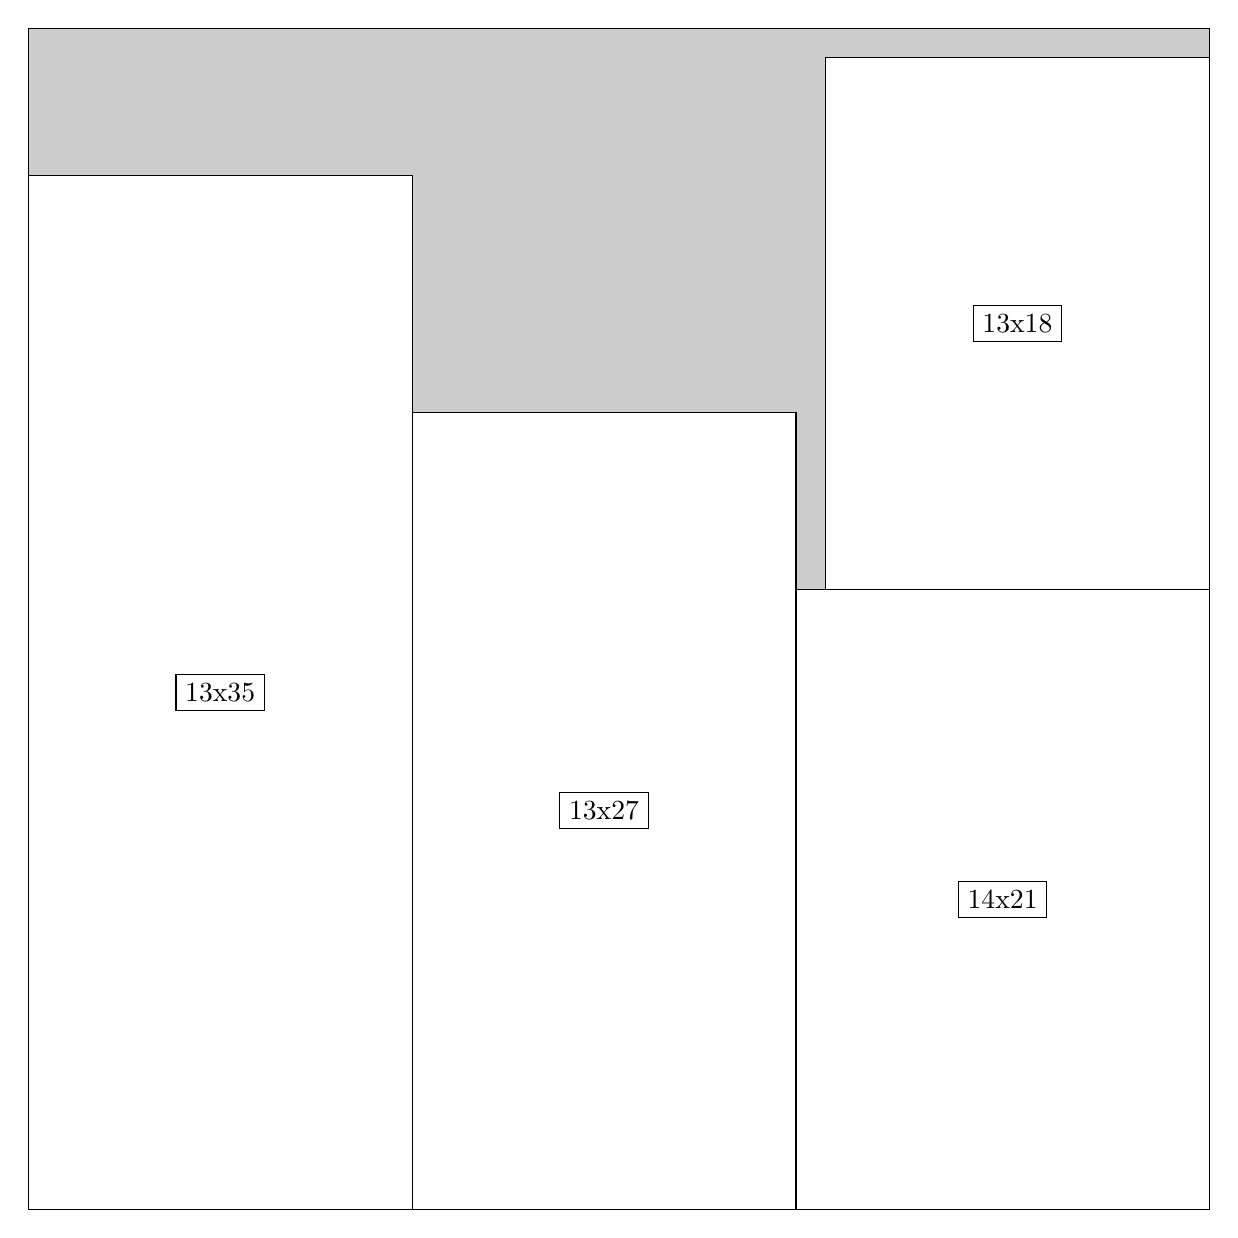
\begin{tikzpicture}[shorten >=1pt,scale=1.0,every node/.style={scale=1.0},->]
\tikzstyle{vertex}=[circle,fill=black!25,minimum size=14pt,inner sep=0pt]
\filldraw[fill=gray!40!white, draw=black] (0,0) rectangle (15.0,15.0);
\foreach \name/\x/\y/\w/\h in {13x35/0.0/0.0/4.875/13.125,13x27/4.875/0.0/4.875/10.125,14x21/9.75/0.0/5.25/7.875,13x18/10.125/7.875/4.875/6.75}
\filldraw[fill=white!40!white, draw=black] (\x,\y) rectangle node[draw] (\name) {\name} ++(\w,\h);
\end{tikzpicture}


w =13 , h =35 , x =0 , y =0 , v =455
\par
w =13 , h =27 , x =13 , y =0 , v =351
\par
w =14 , h =21 , x =26 , y =0 , v =294
\par
w =13 , h =18 , x =27 , y =21 , v =234
\par
\newpage


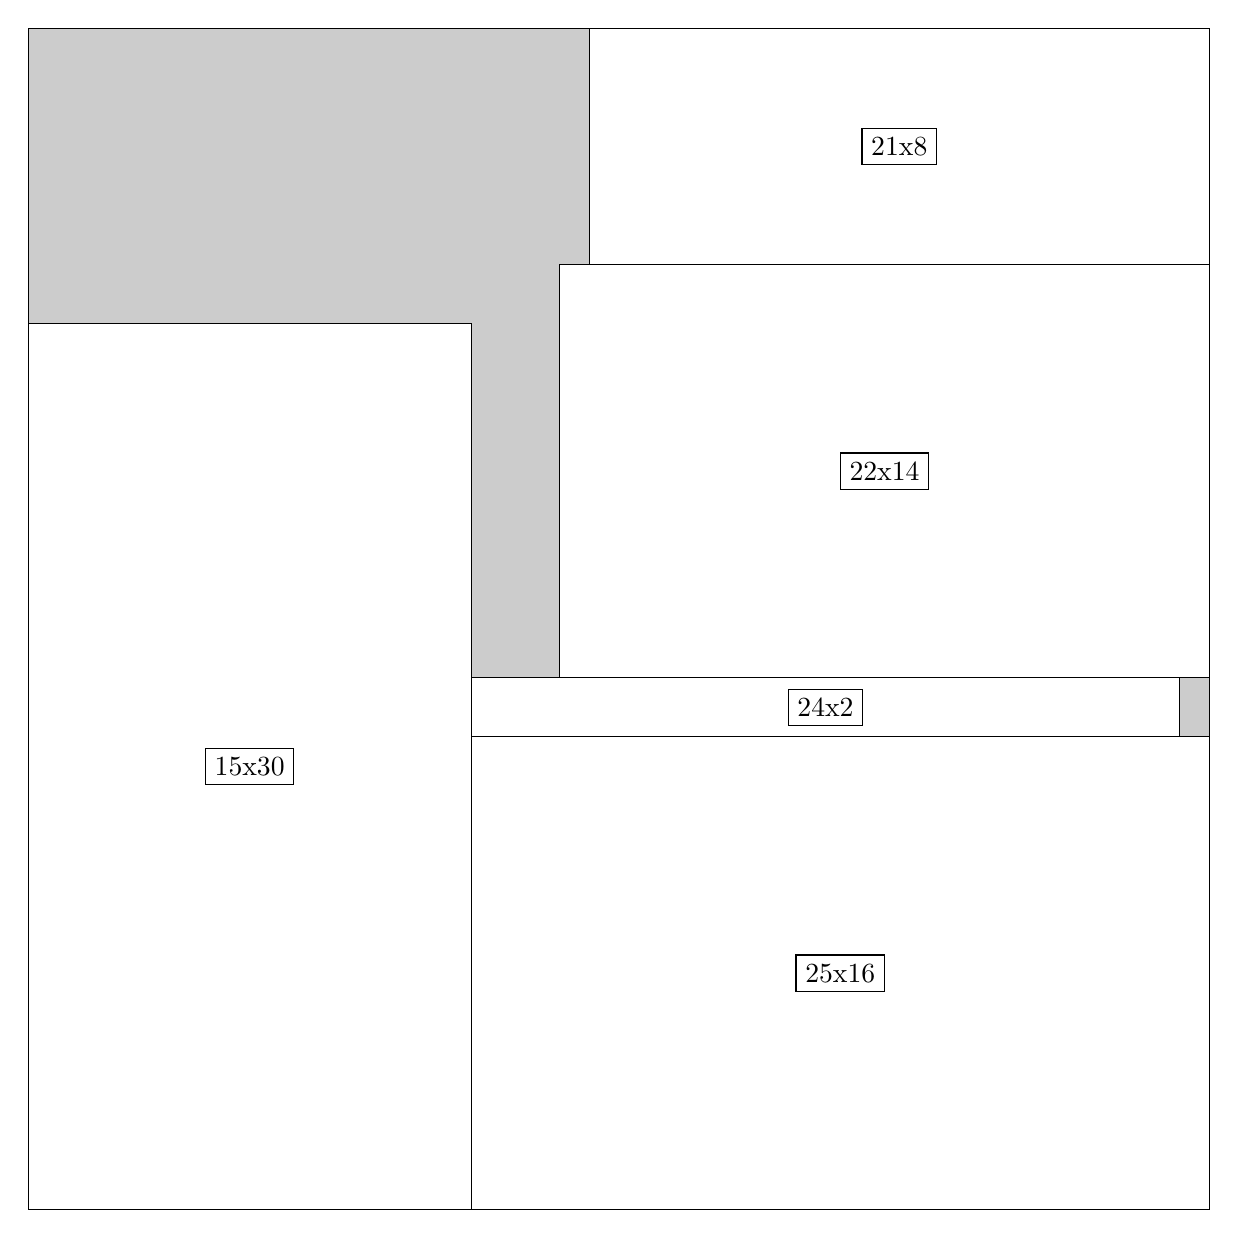
\begin{tikzpicture}[shorten >=1pt,scale=1.0,every node/.style={scale=1.0},->]
\tikzstyle{vertex}=[circle,fill=black!25,minimum size=14pt,inner sep=0pt]
\filldraw[fill=gray!40!white, draw=black] (0,0) rectangle (15.0,15.0);
\foreach \name/\x/\y/\w/\h in {15x30/0.0/0.0/5.625/11.25,25x16/5.625/0.0/9.375/6.0,22x14/6.75/6.75/8.25/5.25,21x8/7.125/12.0/7.875/3.0,24x2/5.625/6.0/9.0/0.75}
\filldraw[fill=white!40!white, draw=black] (\x,\y) rectangle node[draw] (\name) {\name} ++(\w,\h);
\end{tikzpicture}


w =15 , h =30 , x =0 , y =0 , v =450
\par
w =25 , h =16 , x =15 , y =0 , v =400
\par
w =22 , h =14 , x =18 , y =18 , v =308
\par
w =21 , h =8 , x =19 , y =32 , v =168
\par
w =24 , h =2 , x =15 , y =16 , v =48
\par
\newpage


\end{document}